\documentclass[a4paper, 11pt]{memoir}

\usepackage[T1]{fontenc}
\usepackage[utf8]{inputenc}

\usepackage[english]{babel}

\input{smart-thesis/style}
\input{smart-thesis/common-packages}
\input{smart-thesis/common-macros}

\usepackage{lipsum}
\usepackage[table]{xcolor}
\usepackage{minted}

% pgfplots preamble
\usetikzlibrary{arrows.meta}
\usetikzlibrary{backgrounds}
\usepgfplotslibrary{patchplots}
\usepgfplotslibrary{fillbetween}
\pgfplotsset{%
    layers/standard/.define layer set={%
        background,axis background,axis grid,axis ticks,axis lines,axis tick labels,pre main,main,axis descriptions,axis foreground%
    }{
        grid style={/pgfplots/on layer=axis grid},%
        tick style={/pgfplots/on layer=axis ticks},%
        axis line style={/pgfplots/on layer=axis lines},%
        label style={/pgfplots/on layer=axis descriptions},%
        legend style={/pgfplots/on layer=axis descriptions},%
        title style={/pgfplots/on layer=axis descriptions},%
        colorbar style={/pgfplots/on layer=axis descriptions},%
        ticklabel style={/pgfplots/on layer=axis tick labels},%
        axis background@ style={/pgfplots/on layer=axis background},%
        3d box foreground style={/pgfplots/on layer=axis foreground},%
    },
}

\addbibresource{main.bib}

\makeglossaries
\newglossaryentry{transmittance}{
    name=Transmittance,
    description={The transmittance $T \in [0,1]$ is the fraction of light passing straight between two points}
}

\newglossaryentry{radiance}{
    name=Radiance,
    description={The radiance $L$ is the fraction of reflected light}
}

% TODO: Do I need this?
\newglossaryentry{pinhole_camera}{
    name=Pinhole Camera,
    description={Camera model where a given space is projected onto a plane through a point}
}

\newglossaryentry{lambda}{
    name=Lambda,
    description={A lambda function is a function that is not bound to a symbol at compile. Instead it is bound to a variable at runtime or passed directly to a higher order function as an argument}
}

\newglossaryentry{vulkan}{
    name=Vulkan,
    description={A low-level graphics API and standard developed by the Khronos Group}
}

\newglossaryentry{albedo}{
    name=Albedo,
    description={The fraction of light a body reflects diffusely. Value in $[0, 1]$ given separately for each color channel, where $0$ denotes no reflection and $1$ denotes full reflection}
}

\newglossaryentry{simd}{
    name=SIMD,
    description={SIMD (Single Instruction Multiple Data) is a form of parallelism that performs a single operation on multiple pieces of data in parallel on a single CPU}
}

\newglossaryentry{ndc}{
    name=Normalized Device Coordinates,
    description={A coordinate space normalized to $[-1, 1] \times [-1, 1]$}
}

\newglossaryentry{pipelining}{
    name=Pipelining,
    description={Modern CPUs usually have multiple pipeline stages. This means that a new instruction can be submitted to a pipelined unit before the result of the previous instruction is available}
}

\newglossaryentry{latency}{
    name=Latency,
    description={The number of CPU cycles it takes for an instruction's result to be available}
}

\newglossaryentry{throughput}{
    name=Throughput,
    description={The number of CPU cycles it takes, after an instruction is started, until another instruction can be executed}
}

\newglossaryentry{isotropic}{
    name=Isotropic Gaussian,
    description={An isotropic Gaussian has a scalar value as its standard deviation and is affected by it equally in all dimensions}
}


\thesistype{Bachelor Thesis}
\discipline{Computer Science}
\title{Parallel Gaussian Raytracing on the CPU}
\author{Sebastian Dawid}
\institution{Bielefeld University,Technical Faculty,Visual AI for Extended Reality Group}
\supervisors{Prof.\@~Dr.\@~Helge Rhodin,Prof.\@~Dr.-Ing.\@~Ralf M\"oller}

\newcommand*{\erf}{\text{erf}}

\makepagestyle{abs}

% Display the page number in the footer.
\makeevenfoot{abs}{\thepage}{}{}
\makeoddfoot{abs}{}{}{\thepage}

\begin{document}
    \frontmatter
    \smarttitle
    \newpage
    \tableofcontents*

    \clearpage
    \thispagestyle{abs}
    \abstractintoc
    \begin{abstract}
        \lipsum[1]
    \end{abstract}

    \mainmatter
    \chapter{Introduction}

    \section{Gaussian Ray Tracing}
    \label{sec:int_grt}
    %@TODO: propose or describe?
    In their 2015 Paper \citetitle{Rhodin:2015} \cite{Rhodin:2015} Rhodin \etal describe a volumetric image formation
    model based on a parametric density representation $D(\mathbf{x})$ given as the sum of scaled isotropic Guassians
    $\mathcal{G} = \{ G_q \}_q$. The density $D$ is then given as:
    \begin{align}
        D(\mathbf{x}) = \sum_{G_q \in \mathcal{G}} G_q(\mathbf{x})
        \label{eq:density}\\
        G_q(\mathbf{x}) = c_q \cdot \exp{\left( - \frac{\Vert\mathbf{x} - \mu_q\Vert_2^2}{2\sigma_q^2} \right)}
        \label{eq:gaussian}
    \end{align}
    where $c_q$ describes the magnitude, $\mu_q$ the center and $\sigma_q$ the standard deviation of the Gaussian $G_q$.
    Additionally an \gls{albedo} attribute $\mathbf{a}_q$ is defined for each Gaussian to denote its color. This leads
    to the scene representation $\gamma = \{ c_q, \mu_q, \sigma_q, \mathbf{a}_q \}$. The $\gamma$ is omitted from
    $G_q(\mathbf{x})$ for readability and since the parameters are given implicitly via $q$.

    To get the final color of a pixel they determine the amount of light that reaches the camera from each point
    along a ray. For this purpose they determine the \gls{transmittance} $T$ of a point at distance $s$ along a ray from
    a camera position $\mathbf{o}$ in direction $\mathbf{n}$ as:
    \begin{equation}
        T(\mathbf{o}, \mathbf{n}, s, \gamma) = \exp{\left( - \int_0^s D(\mathbf{o} + t\mathbf{n}) dt \right)}
        \label{eq:transmittance}
    \end{equation}

    For the Gaussian density representation the density along a ray $\mathbf{x} = \mathbf{o} + s\mathbf{n}$ through a
    sum of 3D Gaussians is a sum of 1D Gaussians, where the 1D Gaussians are given by inserting the ray into the
    3D Gaussians $G_q$ (\refeq{eq:gaussian}). This results in the form
    $\bar{c} \exp{\left( - \frac{(x - \bar{\mu})^2}{2\bar{\sigma}^2} \right)}$ for the 1D scaled Gaussians, with
    $\bar{\mu} = (\mu - \mathbf{o})^T\mathbf{n}$, $\bar{\sigma} = \sigma$ and
    $\bar{c} = c \cdot \exp{\left( - \frac{(\mu - \mathbf{o})^T(\mu - \mathbf{o}) - \bar{\mu}^2}{2\bar{\sigma}^2} \right)}$.

    The \gls{transmittance} can be expressed analytically using the error function
    $\erf{(x)} = \frac{2}{\sqrt{\pi}}\int_0^s \exp{(-t^2)} dt$ and gaussian form of the density, as follows:
    \begin{equation}
        \begin{aligned}
            T(\mathbf{o}, \mathbf{n}, s, \gamma) &= \exp{\left( -\int_0^s
                \sum_q G_q(\mathbf{o} + t\mathbf{n} ) dt \right)}\\
            &= \exp{\left( \sum_q \frac{\bar{\sigma}_q \bar{c}_q}{\sqrt{\frac{2}{\pi}}}
            \left( \erf{\left( \frac{-\bar{\mu}_q}{\sqrt{2}\bar{\sigma}_q} \right)}
            - \erf{\left( \frac{s - \bar{\mu}_q}{\sqrt{2}\bar{\sigma}_q} \right)} \right) \right)}\\
        \end{aligned}
        \label{eq:transmittance_analytical}
    \end{equation}

    Assuming the elements in the scene emit an equal amount of \gls{radiance}, a ray is shot through each pixel of a virtual
    \gls{pinhole_camera}. The \gls{radiance} can be computed as the product of \gls{transmittance} $T$ (\refeq{eq:transmittance}),
    density $D$ (\refeq{eq:density}), \gls{albedo} $\mathbf{a}$ and the ambient \gls{radiance} $L_e$ integrated along a ray
    $\mathbf{x} = \mathbf{o} + s\mathbf{n}$. They assume the ambient \gls{radiance} is fixed as $L_e = 1$. As such they
    disregard it in the following equation:
    \begin{equation}
        L(\mathbf{o}, \mathbf{n}, \gamma) = \int_0^\infty T(\mathbf{o}, \mathbf{n}, s, \gamma)
            \sum_q G_q(\mathbf{o} + s\mathbf{n})\mathbf{a}_q ds
    \end{equation}
    
    This integral may be approximated with sufficient accuracy by sampling around the mean of each Gaussian $G_q$
    a compact interval $S_q = \{ \bar{\mu}_q + k\lambda_q | k \in K \subset \Z \}$. For their purposes it was sufficient
    to choose $\lambda_q \sim \bar{\sigma}_q$ as the step length:
    \begin{equation}
        \hat{L}(\mathbf{o}, \mathbf{n}, \gamma) = \sum_q \mathbf{a}_q \sum_{s \in S_q}
            \lambda_q T(\mathbf{o}, \mathbf{n}, s, \gamma)G_q(\mathbf{o} + s\mathbf{n})
        \label{eq:radiance}
    \end{equation}

    Rhodin \etal describe that local sampling with $\lambda_q = \bar{\sigma}_q$ and
    $K = \{ -4, -3, \dots, 0 \}$ delivers a good enough approximation.

    \section{Gaussian Splatting}
    %@TODO: describe image formation model (splatting) as laid out in the following pagpers
    \cite{kerbl3Dgaussians}
    \cite{volume_splatting}

    \section{Ray Tracing vs. Splatting}
    %@TODO: What differentiates the two methods? Advantages? Disadvantages?

    \chapter{Optimizations}
    %@TODO: Write introductory paragraph on optimizations
    \section{SIMD}
    %@TODO: Write short introduction on SIMD
    \subsection{Notation}
    To properly rewrite the method as it is laid out in \cite{Rhodin:2015} it is
    necessary to introduce some notation to work with \gls{simd} vectors. This is
    defined in Table~\ref{tab:notation}:
    \begin{table}[h]
        \centering
        \rowcolors{1}{white}{lightgray}
        \begin{tabular}{|c|c|}
            \hline
            Notation & Definition \\
            \hline
            $x^W$ & \gls{simd} vector containing $W$ elements\\
            $x^W_i$ & $i$-th element of \gls{simd} vector $x$\\
            $\mathbf{x}^W$ & \gls{simd} vectors containing $W$ vectors $\mathbf{x} \in \R^n$\\
            $\langle \mathbf{x}^W, \mathbf{y}^W \rangle$ & elementwise inner product of the vectors in $\mathbf{x}$ and $\mathbf{y}$\\
            $[ x ]^W$ & $x$ broadcast to a \gls{simd} vector of $W$ elements\\
            $\odot$ & elementwise multiplication\\
            $\frac{x^W}{y^W}$ & elementwise division\\
            $f^W$ & function that produces a \gls{simd} vector containing $W$ elements\\\hline
        \end{tabular}
        \caption{\gls{simd} Notation}
        \label{tab:notation}
    \end{table}

    \subsection{Approaches}
    \paragraph{Parallel \gls{transmittance}:}
    \label{par:parallel_transmittance}
    \begin{equation}
        \begin{aligned}
            T^W(\mathbf{o}, \mathbf{n}, s, \gamma) &= \exp^W\left( \sum_{m = 0}^{\left\lceil \frac{|\mathcal{G}|}{W} \right\rceil - 1}
            \begin{pmatrix}
                \frac{\bar{\sigma}_{mW}\bar{c}_{mW}}{\sqrt{\frac{2}{\pi}}} \\ \vdots \\\frac{\bar{\sigma}_{(m+1)W-1}\bar{c}_{(m+1)W-1}}{\sqrt{\frac{2}{\pi}}} 
            \end{pmatrix} \right.\\&\left.\odot \begin{pmatrix}
                \erf{\left( \frac{- \bar{\mu}_{mW}}{\sqrt{2}\bar{\sigma}_{mW}} \right) - \erf{\left( \frac{s - \bar{\mu}_{mW}}{\sqrt{2}\bar{\sigma}_{mW}} \right)}} \\
                \vdots \\
               \erf{\left( \frac{- \bar{\mu}_{(m+1)W - 1}}{\sqrt{2}\bar{\sigma}_{(m+1)W - 1}} \right) - \erf{\left( \frac{s - \bar{\mu}_{(m+1)W - 1}}{\sqrt{2}\bar{\sigma}_{(m+1)W - 1}} \right)}} 
            \end{pmatrix}\right)
        \end{aligned}
    \end{equation}
    \begin{equation}
        \hat{L}(\mathbf{o}, \mathbf{n}, \gamma) = \sum_{q} \mathbf{a}_q \sum_{s \in S_q} \lambda_qG_q(\mathbf{o} + s\mathbf{n})\sum_{i = 1}^W T^W_i(\mathbf{o}, \mathbf{n}, s, \gamma)
    \end{equation}

    \paragraph{Parallel \gls{radiance}:}
    \label{par:parallel_radiance}
    The analytical solution to the \gls{transmittance} integral from Eq.~\refeq{eq:transmittance_analytical} can be broadcast
    to operate on \gls{simd} vectors of points on rays parameterized by origins $\mathbf{o}^W$, directions $\mathbf{n}^W$
    and distances $s^W$, as follows:
    \begin{equation}
        \begin{aligned}
            T^W(\mathbf{o}^W, \mathbf{n}^W, s^W, \gamma) = \exp^W\Bigg(& \sum_q \frac{(\bar{\sigma}_q)^W
            (\bar{c}_q)^W}{\left[ \sqrt{\frac{2}{\pi}} \right]^W} \\
            \odot \Bigg(& \erf^W{\left( \frac{-(\bar{\mu}_q)^W}{[ \sqrt{2} ]^W \odot (\bar{\sigma}_q)^W} \right)}\\
            &- \erf^W{\left( \frac{s^W - (\bar{\mu}_q)^W}{[ \sqrt{2} ]^W \odot (\bar{\sigma}_q)^W} \right)} \Bigg) \Bigg) 
        \end{aligned}
        \label{eq:transmittance_broadcast}
    \end{equation}
    with
    \begin{align*}
        \bar{\mu}^W &= \left\langle [ \mu ]^W - \mathbf{o}, \mathbf{n}^W \right\rangle, \bar{\sigma}^W = \left[ \sigma \right]^W\\
        \bar{c}^W &= [c]^W \odot \exp^W{\left( - \frac{\left\langle [\mu]^W - \mathbf{o}^W, [\mu]^W - \mathbf{o}^W \right\rangle
    - \left(\bar{\mu}^W\right)^2}{[2]^W \odot \left(\bar{\sigma}^W\right)^2} \right)}
    \end{align*}

    This version of the \gls{transmittance} equation (\refeq{eq:transmittance_analytical}) allows me to rewrite the \gls{radiance} equation to operate on
    multiple gaussians at the same time as follows:
    \begin{equation}
        \begin{aligned}
            \hat{L}^W(\mathbf{o}, \mathbf{n}, \gamma) &= \sum_{m = 0}^{\left\lceil \frac{|\mathcal{G}|}{W} \right\rceil - 1} \left( \begin{pmatrix}
                \mathbf{a}_{mW}\\ \vdots \\ \mathbf{a}_{(m+1)W - 1}
            \end{pmatrix} \right.\\
            &\odot \sum_{s^W \in S_m} \left( T^W([\mathbf{o}]^W, [\mathbf{n}]^W, s^w, \gamma)\right.\\
            &\odot \left.\left.\begin{pmatrix}
                G_{mW}(\mathbf{o} + s^W_1\mathbf{n})\\ \vdots\\ G_{(m+1)W - 1}(\mathbf{o} + s^W_W\mathbf{n})
            \end{pmatrix}\right)\right)
        \end{aligned}
        \label{eq:radiance_parallel_gaussians}
    \end{equation}
    with
    \[ S_m = \left\{\left. \begin{pmatrix}
        \bar{\mu}_{mW}\\ \vdots\\ \bar{\mu}_{(m+1)W - 1}
    \end{pmatrix} + [k]^W \odot \begin{pmatrix}
        \lambda_{mW}\\ \vdots\\ \lambda_{(m+1)W - 1}
    \end{pmatrix} \,\right|\, k \in K \subset \Z \right\} \]
    and $\bar{\mu}$, $\bar{\sigma}$ and $\bar{c}$ defined the same as in Section~\ref{sec:int_grt}.

    Finally we can collect these results into the final \gls{radiance}:
    \begin{equation}
        \hat{L}(\mathbf{o}, \mathbf{n}, \gamma) = \sum_{i = 1}^W \hat{L}^W_i(\mathbf{o}, \mathbf{n}, \gamma)
        \label{eq:radiance_parallel_final}
    \end{equation}

    \paragraph{Parallel Pixels:}
    \label{par:parallel_pixels}
    Given the broadcast version of the \gls{transmittance} equation (\refeq{eq:transmittance_broadcast}) from before I can broadcast the \gls{radiance} equation to
    calculate the \gls{radiance} for multiple pixels at once:
    \begin{equation}
        \begin{aligned}
            \hat{L}^W(\mathbf{o}^W, \mathbf{n}^W, \gamma) &= \sum_q [ \mathbf{a}_q ]^W \sum_{s \in S_q} \Big(
            [ \lambda_q ]^W \odot T^W(\mathbf{o}^W, \mathbf{n}^W, [ s ]^W, \gamma)\\
            &\odot G_q^W(\mathbf{o}^W + [ s ]^W \odot \mathbf{n}^W) \Big)
        \end{aligned}
        \label{eq:radiance_parallel_pixels}
    \end{equation}

    Note that both the \gls{transmittance} and \gls{radiance} equations still operate on the Gaussians one by one as the
    sums iterate over every Gaussian $G_q \in \mathcal{G}$ individually.

    \section{Tiling}
    %@TODO: describe the tiling method used. note similarities to splatting.
    
    \chapter{Approximations}
    %@TODO: Explain why it is necessary to approximate functions / implement own approximations
    \section{Exponential Function}
    \subsection{Cubic Spline Interpolation}
    \subsection{Bit Hack}
    \cite{fast_exp}
    
    \section{Error Function}
    \subsection{Cubic Spline Interpolation}
    \subsection{Polynomial Approximation}
    \citeauthor{AbraSteg72} give one such approximation in Section 7.1.27 of their \enquote{\citetitle{AbraSteg72}}\cite{AbraSteg72} as:
    \begin{equation}
        \erf{(x)} = 1 - \frac{1}{(1 + ax + bx^2 + cx^3 + dx^4)^4}
    \end{equation}
    with
    \begin{align*}
        a &= 0.278393,\,
        b = 0.230289\\
        c &= 0.000972,\,
        d = 0.078108
    \end{align*}
    
    \chapter{Implementation}
    %@TODO: details TBD
    The source code of the implementation is available at: \href{https://github.com/Sebastian-Dawid/simd-gaussian-ray-tracing}{https://github.com/Sebastian-Dawid/simd-gaussian-ray-tracing}

    To enable cross compilation for different \gls{simd} extentions, here AVX2 and AVX512, I use the T-SIMD library described in \enquote{\citetitle{own_moeller_16_2}} \cite{own_moeller_16_2} by \citeauthor{own_moeller_16_2}.
    
    \chapter{Experiments}
    \section{Approximations}
    \section{Transmittance}
    \section{Full Render}
    Aside from testing singular functions or sections of the program, I have also performed a number of end-to-end tests
    to evaluate the performance improvements of the implemented optimizations in a, close to, real world scenario.
    The tests will be performed on two separate models and evaluate different aspects of the implementation,
    which I will describe in the following sections:
    \subsection{Utah/Newell Teapot}
    \href{https://graphics.stanford.edu/courses/cs148-10-summer/as3/code/as3/teapot.obj}{Model}\footnote{https://graphics.stanford.edu/courses/cs148-10-summer/as3/code/as3/teapot.obj}
    \subsection{Dense Cube}
    
    \chapter{Results and Discussion}
    \section{HPCTOOLKIT}
    \cite{hpc_toolkit}

    The derived metrics used were vector instruction waste and vector instruction efficiency defined as:
    \begin{align}
        \text{waste}(\text{cycles}, \text{instructions}) = 2 \cdot \text{cycles} - \text{instructions} \label{eq:vec_waste}\\
        \text{efficiency}(\text{cycles}, \text{instructions}) = 100 \cdot \frac{\text{instructions}}{2\cdot\text{cycles}} \label{eq:vec_efficiency}
    \end{align}
    which should be based on the exclusive\footnote{An exclusive metric refers to the quantity of the metric measured for that scope
    alone, disregarding nested scopes such as function calls. Reference: HPCTOOLKIT User Manual page 18
    \href{https://hpctoolkit.org/manual/HPCToolkit-users-manual.pdf}{https://hpctoolkit.org/manual/HPCToolkit-users-manual.pdf}}
    \mintinline{c}{PAPI_TOT_CYC} (total cycles) and \mintinline{c}{PAPI_VEC_INS}
    (vector instructions) metrics for the given scopes. HPCToolkit does not include inlined functions in exclusive metrics, which is why \gls{simd}
    instructions and CPU cycles generated by the T-SIMD library would not count towards the exclusive \mintinline{c}{PAPI_VEC_INS} and \mintinline{c}{PAPI_TOT_CYC}
    events. Therefore the derived metrics are calculated using the inclusive metrics. To obtain the final value for the derived metrics the
    value of the derived metrics of the scopes of non T-SIMD functions are subtracted from the value calculated using the inclusive metrics.

    \chapter{Conclusion and Future Work}
    %@TODO: Short recap + what can still be done: anisotropic gaussians, loading models learned via gaussian splatting, more efficient tiling method using SIMD, performance left on the table TBD (see results)

    \appendix
    \chapter{Tables}
    \begin{table}[h]
        \centering
        \rowcolors{1}{white}{lightgray}
        \begin{tabular}{|c|c|}
            \hline
            Mode & Features\\
            1    & Sequential Baseline\\
            2    & Parallel \gls{transmittance}\\
            3    & Parallel \gls{radiance}\\
            4    & Parallel Pixels\\
            5    & Sequential + Tiling\\
            6    & Parallel \gls{transmittance} + Tiling\\
            7    & Parallel \gls{radiance} + Tiling\\
            8    & Parallel Pixels + Tiling\\
            st   & Single Threaded\\
            mt   & Multi Threaded\\
            \hline
        \end{tabular}
        \caption{Modes}
        \label{tab:exec_modes}
    \end{table}
    \begin{table}[h]
        \centering
        \rowcolors{1}{white}{lightgray}
        \begin{tabular}{|c | c | c|}
            \hline
            Mode & GCC                               & GCC-SVML\\\hline
            1 st & $\sim27.6$ min ($1656410.9$ ms)     & -\\
            2 st & $\sim111.34$ sec ($111344.03$ ms) & $\sim94.79$ sec ($95795.984$ ms)\\
            3 st & $\sim78.3$ sec ($78304.445$ ms)   & $\sim66.08$ sec ($66084.97$ ms)\\
            4 st & $\sim80.89$ sec ($80892.84$ ms)   & $\sim60.61$ sec ($60613.37$ ms)\\
            5 st & $\sim15.31$ sec ($15312.966$ ms)  & $\sim12.44$ sec ($12438.755$ ms)\\
            6 st & $\sim1.72$ sec ($1718.0503$ ms)   & $\sim1.21$ sec ($1208.4868$ ms)\\
            7 st & $\sim0.84$ sec ($835.83826$ ms)   & $\sim0.72$ sec ($721.6306$ ms)\\
            8 st & $\sim0.77$ sec ($768.4175$ ms)    & $\sim0.59$ sec ($594.68164$ ms)\\\hline\hline
            5 mt & $\sim0.582$ sec ($582.271$ ms)    & $\sim0.502$ sec ($502.71063$ ms)\\
            6 mt & $\sim0.085$ sec ($84.843185$ ms)  & $\sim0.068$ sec ($67.78539$ ms)\\
            7 mt & $\sim0.057$ sec ($57.257492$ ms)  & $\sim0.051$ sec ($51.06643$ ms)\\
            8 mt & $\sim0.052$ sec ($52.194233$ ms)  & $\sim0.046$ sec ($45.902195$ ms)\\
            \hline
        \end{tabular}
        \caption{Runtime of rendering the dense cube based on SVML usage and mode using AVX512.}
        \label{tab:perf_dense_cube_avx512_gcc}
    \end{table}

    \begin{table}[h]
        \centering
        \rowcolors{1}{white}{lightgray}
        \begin{tabular}{|c|c|c|c|c|}
            \hline
            Mode & \gls{radiance}             & \gls{transmittance}          & $\erf$                      & $\exp$\\\hline
            1 st & & & &\\
            2 st & & & &\\
            3 st & & & &\\
            4 st & & & &\\
            5 st & & & &\\
            6 st & & & &\\
            7 st & $3.8 \cdot 10^7$ ($0.9\%$) & $1.15 \cdot 10^9$ ($28.4\%$) & $1.14 \cdot 10^8$ ($2.8\%$) & $4.0 \cdot 10^6$ ($0.1\%$)\\
            8 st & & & &\\\hline\hline
            5 mt & & & &\\
            6 mt & & & &\\
            7 mt & & $3.96 \cdot 10^8$ ($4.4\%$) & &\\
            8 mt & & & &\\
            \hline
        \end{tabular}
        \caption{Clang: Vector Instruction Waste (\% of total) by Mode}
        \label{tab:clang_vec_waste}
    \end{table}
    \begin{table}[h]
        \centering
        \rowcolors{1}{white}{lightgray}
        \begin{tabular}{|c|c|c|c|c|}
            \hline
            Mode & \gls{radiance} & \gls{transmittance} & $\erf$   & $\exp$\\\hline
            1 st & & & &\\
            2 st & & & &\\
            3 st & & & &\\
            4 st & & & &\\
            5 st & & & &\\
            6 st & & & &\\
            7 st & $5.0\%$        & $53.78\%$           & $25.0\%$ & - \\
            8 st & & & &\\\hline\hline
            5 mt & & & &\\
            6 mt & & & &\\
            7 mt & & $31.25\%$ & &\\
            8 mt & & & &\\
            \hline
        \end{tabular}
        \caption{Clang: Vector Instruction Efficiency by Mode}
        \label{tab:clang_vec_efficiency}
    \end{table}

    \chapter{Figures}
    \begin{figure}[h]
        \centering
        % Recommended preamble:
% \usetikzlibrary{arrows.meta}
% \usetikzlibrary{backgrounds}
% \usepgfplotslibrary{patchplots}
% \usepgfplotslibrary{fillbetween}
% \pgfplotsset{%
%     layers/standard/.define layer set={%
%         background,axis background,axis grid,axis ticks,axis lines,axis tick labels,pre main,main,axis descriptions,axis foreground%
%     }{
%         grid style={/pgfplots/on layer=axis grid},%
%         tick style={/pgfplots/on layer=axis ticks},%
%         axis line style={/pgfplots/on layer=axis lines},%
%         label style={/pgfplots/on layer=axis descriptions},%
%         legend style={/pgfplots/on layer=axis descriptions},%
%         title style={/pgfplots/on layer=axis descriptions},%
%         colorbar style={/pgfplots/on layer=axis descriptions},%
%         ticklabel style={/pgfplots/on layer=axis tick labels},%
%         axis background@ style={/pgfplots/on layer=axis background},%
%         3d box foreground style={/pgfplots/on layer=axis foreground},%
%     },
% }

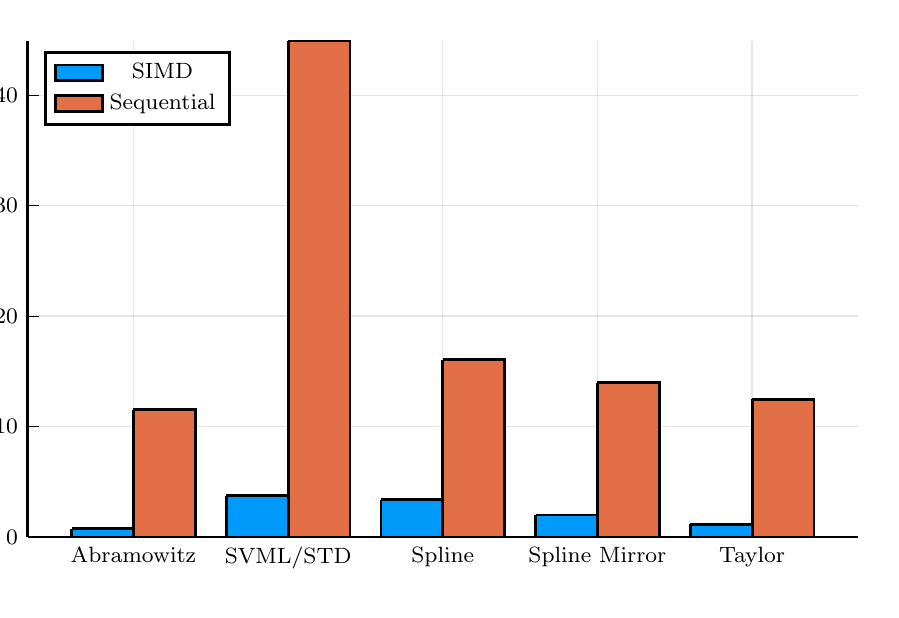
\begin{tikzpicture}[/tikz/background rectangle/.style={fill={rgb,1:red,1.0;green,1.0;blue,1.0}, fill opacity={1.0}, draw opacity={1.0}}, show background rectangle, trim axis left]
\begin{axis}[point meta max={nan}, point meta min={nan}, legend cell align={left}, legend columns={1}, title={}, title style={at={{(0.5,1)}}, anchor={south}, font={{\fontsize{14 pt}{18.2 pt}\selectfont}}, color={rgb,1:red,0.0;green,0.0;blue,0.0}, draw opacity={1.0}, rotate={0.0}, align={center}}, legend style={color={rgb,1:red,0.0;green,0.0;blue,0.0}, draw opacity={1.0}, line width={1}, solid, fill={rgb,1:red,1.0;green,1.0;blue,1.0}, fill opacity={1.0}, text opacity={1.0}, font={{\fontsize{8 pt}{10.4 pt}\selectfont}}, text={rgb,1:red,0.0;green,0.0;blue,0.0}, cells={anchor={center}}, at={(0.02, 0.98)}, anchor={north west}}, axis background/.style={fill={rgb,1:red,1.0;green,1.0;blue,1.0}, opacity={1.0}}, anchor={north west}, xshift={1.0mm}, yshift={-1.0mm}, width=\textwidth, height=0.65*\textwidth, scaled x ticks={false}, xlabel={}, x tick style={color={rgb,1:red,0.0;green,0.0;blue,0.0}, opacity={1.0}}, x tick label style={color={rgb,1:red,0.0;green,0.0;blue,0.0}, opacity={1.0}, rotate={0}}, xlabel style={at={(ticklabel cs:0.5)}, anchor=near ticklabel, at={{(ticklabel cs:0.5)}}, anchor={near ticklabel}, font={{\fontsize{11 pt}{14.3 pt}\selectfont}}, color={rgb,1:red,0.0;green,0.0;blue,0.0}, draw opacity={1.0}, rotate={0.0}}, xmajorgrids={true}, xmin={-0.18392000000000008}, xmax={5.1839200000000005}, xticklabels={{Abramowitz,SVML/STD,Spline,Spline Mirror,Taylor}}, xtick={{0.5,1.5,2.5,3.5,4.5}}, xtick align={inside}, xticklabel style={font={{\fontsize{8 pt}{10.4 pt}\selectfont}}, color={rgb,1:red,0.0;green,0.0;blue,0.0}, draw opacity={1.0}, rotate={0.0}}, x grid style={color={rgb,1:red,0.0;green,0.0;blue,0.0}, draw opacity={0.1}, line width={0.5}, solid}, axis x line*={left}, x axis line style={color={rgb,1:red,0.0;green,0.0;blue,0.0}, draw opacity={1.0}, line width={1}, solid}, scaled y ticks={false}, ylabel={avg. cycles}, y tick style={color={rgb,1:red,0.0;green,0.0;blue,0.0}, opacity={1.0}}, y tick label style={color={rgb,1:red,0.0;green,0.0;blue,0.0}, opacity={1.0}, rotate={0}}, ylabel style={at={(ticklabel cs:0.5)}, anchor=near ticklabel, at={{(ticklabel cs:0.5)}}, anchor={near ticklabel}, font={{\fontsize{11 pt}{14.3 pt}\selectfont}}, color={rgb,1:red,0.0;green,0.0;blue,0.0}, draw opacity={1.0}, rotate={0.0}}, ymajorgrids={true}, ymin={0.0}, ymax={44.92094559225225}, yticklabels={{$0$,$10$,$20$,$30$,$40$}}, ytick={{0.0,10.0,20.0,30.0,40.0}}, ytick align={inside}, yticklabel style={font={{\fontsize{8 pt}{10.4 pt}\selectfont}}, color={rgb,1:red,0.0;green,0.0;blue,0.0}, draw opacity={1.0}, rotate={0.0}}, y grid style={color={rgb,1:red,0.0;green,0.0;blue,0.0}, draw opacity={0.1}, line width={0.5}, solid}, axis y line*={left}, y axis line style={color={rgb,1:red,0.0;green,0.0;blue,0.0}, draw opacity={1.0}, line width={1}, solid}, colorbar={false}]
    \addplot[color={rgb,1:red,0.0;green,0.0;blue,0.0}, name path={1}, area legend, fill={rgb,1:red,0.0;green,0.6056;blue,0.9787}, fill opacity={1.0}, draw opacity={1.0}, line width={1}, solid]
        table[row sep={\\}]
        {
            \\
            0.09999999999999998  0.7409533367352013  \\
            0.09999999999999998  0.0  \\
            0.5  0.0  \\
            0.5  0.7409533367352013  \\
            0.09999999999999998  0.7409533367352013  \\
        }
        ;
    \addlegendentry {SIMD}
    \addplot[color={rgb,1:red,0.0;green,0.0;blue,0.0}, name path={1}, area legend, fill={rgb,1:red,0.0;green,0.6056;blue,0.9787}, fill opacity={1.0}, draw opacity={1.0}, line width={1}, solid, forget plot]
        table[row sep={\\}]
        {
            \\
            1.1  3.7526630939523598  \\
            1.1  0.0  \\
            1.5  0.0  \\
            1.5  3.7526630939523598  \\
            1.1  3.7526630939523598  \\
        }
        ;
    \addplot[color={rgb,1:red,0.0;green,0.0;blue,0.0}, name path={1}, area legend, fill={rgb,1:red,0.0;green,0.6056;blue,0.9787}, fill opacity={1.0}, draw opacity={1.0}, line width={1}, solid, forget plot]
        table[row sep={\\}]
        {
            \\
            2.1  3.388426347695305  \\
            2.1  0.0  \\
            2.5000000000000004  0.0  \\
            2.5000000000000004  3.388426347695305  \\
            2.1  3.388426347695305  \\
        }
        ;
    \addplot[color={rgb,1:red,0.0;green,0.0;blue,0.0}, name path={1}, area legend, fill={rgb,1:red,0.0;green,0.6056;blue,0.9787}, fill opacity={1.0}, draw opacity={1.0}, line width={1}, solid, forget plot]
        table[row sep={\\}]
        {
            \\
            3.1  1.9993334294787894  \\
            3.1  0.0  \\
            3.5000000000000004  0.0  \\
            3.5000000000000004  1.9993334294787894  \\
            3.1  1.9993334294787894  \\
        }
        ;
    \addplot[color={rgb,1:red,0.0;green,0.0;blue,0.0}, name path={1}, area legend, fill={rgb,1:red,0.0;green,0.6056;blue,0.9787}, fill opacity={1.0}, draw opacity={1.0}, line width={1}, solid, forget plot]
        table[row sep={\\}]
        {
            \\
            4.1  1.1576248534897213  \\
            4.1  0.0  \\
            4.5  0.0  \\
            4.5  1.1576248534897213  \\
            4.1  1.1576248534897213  \\
        }
        ;
    \addplot[color={rgb,1:red,0.0;green,0.6056;blue,0.9787}, name path={2}, only marks, draw opacity={1.0}, line width={0}, solid, mark={*}, mark size={0.0 pt}, mark repeat={1}, mark options={color={rgb,1:red,0.0;green,0.0;blue,0.0}, draw opacity={0.0}, fill={rgb,1:red,0.0;green,0.6056;blue,0.9787}, fill opacity={0.0}, line width={0.75}, rotate={0}, solid}, forget plot]
        table[row sep={\\}]
        {
            \\
            0.3  0.7409533367352013  \\
            1.3  3.7526630939523598  \\
            2.3000000000000003  3.388426347695305  \\
            3.3000000000000003  1.9993334294787894  \\
            4.3  1.1576248534897213  \\
        }
        ;
    \addplot[color={rgb,1:red,0.0;green,0.0;blue,0.0}, name path={3}, area legend, fill={rgb,1:red,0.8889;green,0.4356;blue,0.2781}, fill opacity={1.0}, draw opacity={1.0}, line width={1}, solid]
        table[row sep={\\}]
        {
            \\
            0.49999999999999994  11.52229665862018  \\
            0.49999999999999994  0.0  \\
            0.8999999999999999  0.0  \\
            0.8999999999999999  11.52229665862018  \\
            0.49999999999999994  11.52229665862018  \\
        }
        ;
    \addlegendentry {Sequential}
    \addplot[color={rgb,1:red,0.0;green,0.0;blue,0.0}, name path={3}, area legend, fill={rgb,1:red,0.8889;green,0.4356;blue,0.2781}, fill opacity={1.0}, draw opacity={1.0}, line width={1}, solid, forget plot]
        table[row sep={\\}]
        {
            \\
            1.5000000000000002  44.92094559225225  \\
            1.5000000000000002  0.0  \\
            1.9000000000000001  0.0  \\
            1.9000000000000001  44.92094559225225  \\
            1.5000000000000002  44.92094559225225  \\
        }
        ;
    \addplot[color={rgb,1:red,0.0;green,0.0;blue,0.0}, name path={3}, area legend, fill={rgb,1:red,0.8889;green,0.4356;blue,0.2781}, fill opacity={1.0}, draw opacity={1.0}, line width={1}, solid, forget plot]
        table[row sep={\\}]
        {
            \\
            2.5  16.071793031829063  \\
            2.5  0.0  \\
            2.9000000000000004  0.0  \\
            2.9000000000000004  16.071793031829063  \\
            2.5  16.071793031829063  \\
        }
        ;
    \addplot[color={rgb,1:red,0.0;green,0.0;blue,0.0}, name path={3}, area legend, fill={rgb,1:red,0.8889;green,0.4356;blue,0.2781}, fill opacity={1.0}, draw opacity={1.0}, line width={1}, solid, forget plot]
        table[row sep={\\}]
        {
            \\
            3.5  13.983863662740116  \\
            3.5  0.0  \\
            3.9000000000000004  0.0  \\
            3.9000000000000004  13.983863662740116  \\
            3.5  13.983863662740116  \\
        }
        ;
    \addplot[color={rgb,1:red,0.0;green,0.0;blue,0.0}, name path={3}, area legend, fill={rgb,1:red,0.8889;green,0.4356;blue,0.2781}, fill opacity={1.0}, draw opacity={1.0}, line width={1}, solid, forget plot]
        table[row sep={\\}]
        {
            \\
            4.5  12.46172143390689  \\
            4.5  0.0  \\
            4.9  0.0  \\
            4.9  12.46172143390689  \\
            4.5  12.46172143390689  \\
        }
        ;
    \addplot[color={rgb,1:red,0.8889;green,0.4356;blue,0.2781}, name path={4}, only marks, draw opacity={1.0}, line width={0}, solid, mark={*}, mark size={0.0 pt}, mark repeat={1}, mark options={color={rgb,1:red,0.0;green,0.0;blue,0.0}, draw opacity={0.0}, fill={rgb,1:red,0.8889;green,0.4356;blue,0.2781}, fill opacity={0.0}, line width={0.75}, rotate={0}, solid}, forget plot]
        table[row sep={\\}]
        {
            \\
            0.7  11.52229665862018  \\
            1.7000000000000002  44.92094559225225  \\
            2.7  16.071793031829063  \\
            3.7  13.983863662740116  \\
            4.7  12.46172143390689  \\
        }
        ;
\end{axis}
\end{tikzpicture}

        \caption{Cycles to calculate $n$ values of $\erf$.}
    \end{figure}
    \begin{figure}[h]
        \centering
        % Recommended preamble:
% \usetikzlibrary{arrows.meta}
% \usetikzlibrary{backgrounds}
% \usepgfplotslibrary{patchplots}
% \usepgfplotslibrary{fillbetween}
% \pgfplotsset{%
%     layers/standard/.define layer set={%
%         background,axis background,axis grid,axis ticks,axis lines,axis tick labels,pre main,main,axis descriptions,axis foreground%
%     }{
%         grid style={/pgfplots/on layer=axis grid},%
%         tick style={/pgfplots/on layer=axis ticks},%
%         axis line style={/pgfplots/on layer=axis lines},%
%         label style={/pgfplots/on layer=axis descriptions},%
%         legend style={/pgfplots/on layer=axis descriptions},%
%         title style={/pgfplots/on layer=axis descriptions},%
%         colorbar style={/pgfplots/on layer=axis descriptions},%
%         ticklabel style={/pgfplots/on layer=axis tick labels},%
%         axis background@ style={/pgfplots/on layer=axis background},%
%         3d box foreground style={/pgfplots/on layer=axis foreground},%
%     },
% }

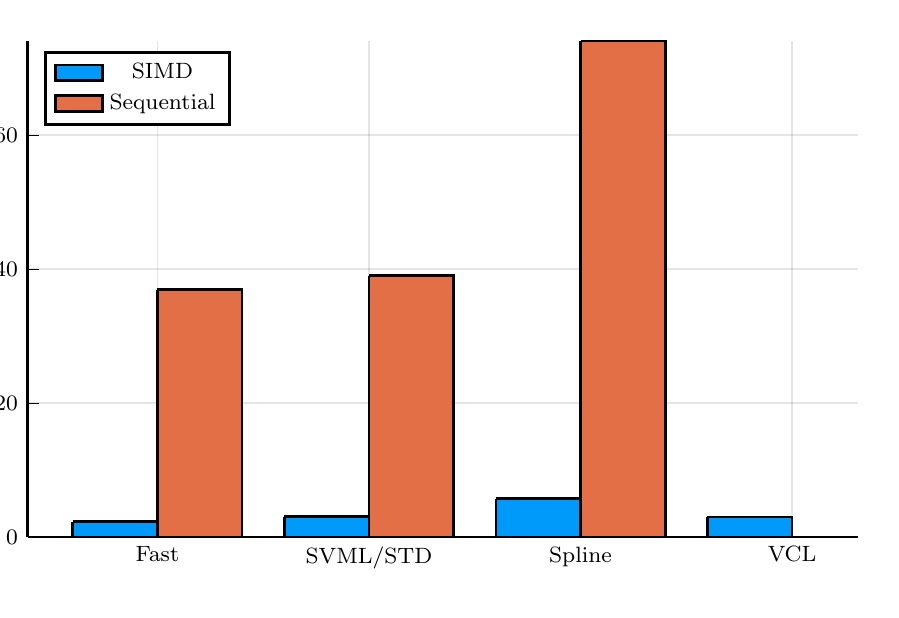
\begin{tikzpicture}[/tikz/background rectangle/.style={fill={rgb,1:red,1.0;green,1.0;blue,1.0}, fill opacity={1.0}, draw opacity={1.0}}, show background rectangle, trim axis left]
\begin{axis}[point meta max={nan}, point meta min={nan}, legend cell align={left}, legend columns={1}, title={}, title style={at={{(0.5,1)}}, anchor={south}, font={{\fontsize{14 pt}{18.2 pt}\selectfont}}, color={rgb,1:red,0.0;green,0.0;blue,0.0}, draw opacity={1.0}, rotate={0.0}, align={center}}, legend style={color={rgb,1:red,0.0;green,0.0;blue,0.0}, draw opacity={1.0}, line width={1}, solid, fill={rgb,1:red,1.0;green,1.0;blue,1.0}, fill opacity={1.0}, text opacity={1.0}, font={{\fontsize{8 pt}{10.4 pt}\selectfont}}, text={rgb,1:red,0.0;green,0.0;blue,0.0}, cells={anchor={center}}, at={(0.02, 0.98)}, anchor={north west}}, axis background/.style={fill={rgb,1:red,1.0;green,1.0;blue,1.0}, opacity={1.0}}, anchor={north west}, xshift={1.0mm}, yshift={-1.0mm}, width=\textwidth, height=0.65*\textwidth, scaled x ticks={false}, xlabel={}, x tick style={color={rgb,1:red,0.0;green,0.0;blue,0.0}, opacity={1.0}}, x tick label style={color={rgb,1:red,0.0;green,0.0;blue,0.0}, opacity={1.0}, rotate={0}}, xlabel style={at={(ticklabel cs:0.5)}, anchor=near ticklabel, at={{(ticklabel cs:0.5)}}, anchor={near ticklabel}, font={{\fontsize{11 pt}{14.3 pt}\selectfont}}, color={rgb,1:red,0.0;green,0.0;blue,0.0}, draw opacity={1.0}, rotate={0.0}}, xmajorgrids={true}, xmin={-0.11305999999999994}, xmax={3.8110600000000003}, xticklabels={{Fast,SVML/STD,Spline,VCL}}, xtick={{0.5,1.5,2.5,3.5}}, xtick align={inside}, xticklabel style={font={{\fontsize{8 pt}{10.4 pt}\selectfont}}, color={rgb,1:red,0.0;green,0.0;blue,0.0}, draw opacity={1.0}, rotate={0.0}}, x grid style={color={rgb,1:red,0.0;green,0.0;blue,0.0}, draw opacity={0.1}, line width={0.5}, solid}, axis x line*={left}, x axis line style={color={rgb,1:red,0.0;green,0.0;blue,0.0}, draw opacity={1.0}, line width={1}, solid}, scaled y ticks={false}, ylabel={avg. cycles}, y tick style={color={rgb,1:red,0.0;green,0.0;blue,0.0}, opacity={1.0}}, y tick label style={color={rgb,1:red,0.0;green,0.0;blue,0.0}, opacity={1.0}, rotate={0}}, ylabel style={at={(ticklabel cs:0.5)}, anchor=near ticklabel, at={{(ticklabel cs:0.5)}}, anchor={near ticklabel}, font={{\fontsize{11 pt}{14.3 pt}\selectfont}}, color={rgb,1:red,0.0;green,0.0;blue,0.0}, draw opacity={1.0}, rotate={0.0}}, ymajorgrids={true}, ymin={0.0}, ymax={74.04927}, yticklabels={{$0$,$20$,$40$,$60$}}, ytick={{0.0,20.0,40.0,60.0}}, ytick align={inside}, yticklabel style={font={{\fontsize{8 pt}{10.4 pt}\selectfont}}, color={rgb,1:red,0.0;green,0.0;blue,0.0}, draw opacity={1.0}, rotate={0.0}}, y grid style={color={rgb,1:red,0.0;green,0.0;blue,0.0}, draw opacity={0.1}, line width={0.5}, solid}, axis y line*={left}, y axis line style={color={rgb,1:red,0.0;green,0.0;blue,0.0}, draw opacity={1.0}, line width={1}, solid}, colorbar={false}]
    \addplot[color={rgb,1:red,0.0;green,0.0;blue,0.0}, name path={5}, area legend, fill={rgb,1:red,0.0;green,0.6056;blue,0.9787}, fill opacity={1.0}, draw opacity={1.0}, line width={1}, solid]
        table[row sep={\\}]
        {
            \\
            0.09999999999999998  2.2899725  \\
            0.09999999999999998  0.0  \\
            0.5  0.0  \\
            0.5  2.2899725  \\
            0.09999999999999998  2.2899725  \\
        }
        ;
    \addlegendentry {SIMD}
    \addplot[color={rgb,1:red,0.0;green,0.0;blue,0.0}, name path={5}, area legend, fill={rgb,1:red,0.0;green,0.6056;blue,0.9787}, fill opacity={1.0}, draw opacity={1.0}, line width={1}, solid, forget plot]
        table[row sep={\\}]
        {
            \\
            1.1  3.0422134  \\
            1.1  0.0  \\
            1.5  0.0  \\
            1.5  3.0422134  \\
            1.1  3.0422134  \\
        }
        ;
    \addplot[color={rgb,1:red,0.0;green,0.0;blue,0.0}, name path={5}, area legend, fill={rgb,1:red,0.0;green,0.6056;blue,0.9787}, fill opacity={1.0}, draw opacity={1.0}, line width={1}, solid, forget plot]
        table[row sep={\\}]
        {
            \\
            2.1  5.7201223  \\
            2.1  0.0  \\
            2.5000000000000004  0.0  \\
            2.5000000000000004  5.7201223  \\
            2.1  5.7201223  \\
        }
        ;
    \addplot[color={rgb,1:red,0.0;green,0.0;blue,0.0}, name path={5}, area legend, fill={rgb,1:red,0.0;green,0.6056;blue,0.9787}, fill opacity={1.0}, draw opacity={1.0}, line width={1}, solid, forget plot]
        table[row sep={\\}]
        {
            \\
            3.1  3.0022936  \\
            3.1  0.0  \\
            3.5000000000000004  0.0  \\
            3.5000000000000004  3.0022936  \\
            3.1  3.0022936  \\
        }
        ;
    \addplot[color={rgb,1:red,0.0;green,0.6056;blue,0.9787}, name path={6}, only marks, draw opacity={1.0}, line width={0}, solid, mark={*}, mark size={0.0 pt}, mark repeat={1}, mark options={color={rgb,1:red,0.0;green,0.0;blue,0.0}, draw opacity={0.0}, fill={rgb,1:red,0.0;green,0.6056;blue,0.9787}, fill opacity={0.0}, line width={0.75}, rotate={0}, solid}, forget plot]
        table[row sep={\\}]
        {
            \\
            0.3  2.2899725  \\
            1.3  3.0422134  \\
            2.3000000000000003  5.7201223  \\
            3.3000000000000003  3.0022936  \\
        }
        ;
    \addplot[color={rgb,1:red,0.0;green,0.0;blue,0.0}, name path={7}, area legend, fill={rgb,1:red,0.8889;green,0.4356;blue,0.2781}, fill opacity={1.0}, draw opacity={1.0}, line width={1}, solid]
        table[row sep={\\}]
        {
            \\
            0.49999999999999994  36.946297  \\
            0.49999999999999994  0.0  \\
            0.8999999999999999  0.0  \\
            0.8999999999999999  36.946297  \\
            0.49999999999999994  36.946297  \\
        }
        ;
    \addlegendentry {Sequential}
    \addplot[color={rgb,1:red,0.0;green,0.0;blue,0.0}, name path={7}, area legend, fill={rgb,1:red,0.8889;green,0.4356;blue,0.2781}, fill opacity={1.0}, draw opacity={1.0}, line width={1}, solid, forget plot]
        table[row sep={\\}]
        {
            \\
            1.5000000000000002  39.033577  \\
            1.5000000000000002  0.0  \\
            1.9000000000000001  0.0  \\
            1.9000000000000001  39.033577  \\
            1.5000000000000002  39.033577  \\
        }
        ;
    \addplot[color={rgb,1:red,0.0;green,0.0;blue,0.0}, name path={7}, area legend, fill={rgb,1:red,0.8889;green,0.4356;blue,0.2781}, fill opacity={1.0}, draw opacity={1.0}, line width={1}, solid, forget plot]
        table[row sep={\\}]
        {
            \\
            2.5  74.04927  \\
            2.5  0.0  \\
            2.9000000000000004  0.0  \\
            2.9000000000000004  74.04927  \\
            2.5  74.04927  \\
        }
        ;
    \addplot[color={rgb,1:red,0.8889;green,0.4356;blue,0.2781}, name path={8}, only marks, draw opacity={1.0}, line width={0}, solid, mark={*}, mark size={0.0 pt}, mark repeat={1}, mark options={color={rgb,1:red,0.0;green,0.0;blue,0.0}, draw opacity={0.0}, fill={rgb,1:red,0.8889;green,0.4356;blue,0.2781}, fill opacity={0.0}, line width={0.75}, rotate={0}, solid}, forget plot]
        table[row sep={\\}]
        {
            \\
            0.7  36.946297  \\
            1.7000000000000002  39.033577  \\
            2.7  74.04927  \\
        }
        ;
\end{axis}
\end{tikzpicture}

        \caption{Cycles to calculate $n$ values of $\exp$.}
    \end{figure}
    
    \begin{figure}[h]
        \centering
        % Recommended preamble:
% \usetikzlibrary{arrows.meta}
% \usetikzlibrary{backgrounds}
% \usepgfplotslibrary{patchplots}
% \usepgfplotslibrary{fillbetween}
% \pgfplotsset{%
%     layers/standard/.define layer set={%
%         background,axis background,axis grid,axis ticks,axis lines,axis tick labels,pre main,main,axis descriptions,axis foreground%
%     }{
%         grid style={/pgfplots/on layer=axis grid},%
%         tick style={/pgfplots/on layer=axis ticks},%
%         axis line style={/pgfplots/on layer=axis lines},%
%         label style={/pgfplots/on layer=axis descriptions},%
%         legend style={/pgfplots/on layer=axis descriptions},%
%         title style={/pgfplots/on layer=axis descriptions},%
%         colorbar style={/pgfplots/on layer=axis descriptions},%
%         ticklabel style={/pgfplots/on layer=axis tick labels},%
%         axis background@ style={/pgfplots/on layer=axis background},%
%         3d box foreground style={/pgfplots/on layer=axis foreground},%
%     },
% }

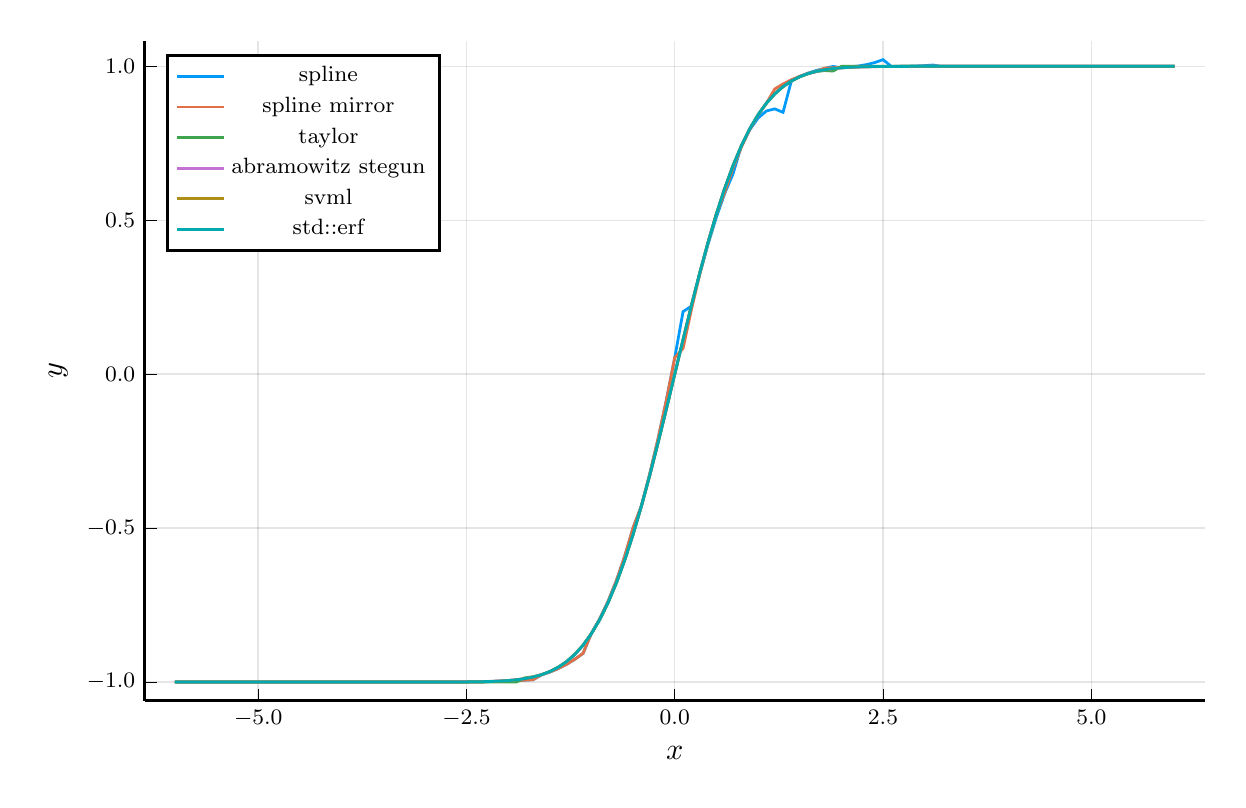
\begin{tikzpicture}[/tikz/background rectangle/.style={fill={rgb,1:red,1.0;green,1.0;blue,1.0}, fill opacity={1.0}, draw opacity={1.0}}, show background rectangle]
\begin{axis}[point meta max={nan}, point meta min={nan}, legend cell align={left}, legend columns={1}, title={}, title style={at={{(0.5,1)}}, anchor={south}, font={{\fontsize{14 pt}{18.2 pt}\selectfont}}, color={rgb,1:red,0.0;green,0.0;blue,0.0}, draw opacity={1.0}, rotate={0.0}, align={center}}, legend style={color={rgb,1:red,0.0;green,0.0;blue,0.0}, draw opacity={1.0}, line width={1}, solid, fill={rgb,1:red,1.0;green,1.0;blue,1.0}, fill opacity={1.0}, text opacity={1.0}, font={{\fontsize{8 pt}{10.4 pt}\selectfont}}, text={rgb,1:red,0.0;green,0.0;blue,0.0}, cells={anchor={center}}, at={(0.02, 0.98)}, anchor={north west}}, axis background/.style={fill={rgb,1:red,1.0;green,1.0;blue,1.0}, opacity={1.0}}, anchor={north west}, xshift={1.0mm}, yshift={-1.0mm}, width={150.4mm}, height={99.6mm}, scaled x ticks={false}, xlabel={$x$}, x tick style={color={rgb,1:red,0.0;green,0.0;blue,0.0}, opacity={1.0}}, x tick label style={color={rgb,1:red,0.0;green,0.0;blue,0.0}, opacity={1.0}, rotate={0}}, xlabel style={at={(ticklabel cs:0.5)}, anchor=near ticklabel, at={{(ticklabel cs:0.5)}}, anchor={near ticklabel}, font={{\fontsize{11 pt}{14.3 pt}\selectfont}}, color={rgb,1:red,0.0;green,0.0;blue,0.0}, draw opacity={1.0}, rotate={0.0}}, xmajorgrids={true}, xmin={-6.359999799000001}, xmax={6.359993099}, xticklabels={{$-5.0$,$-2.5$,$0.0$,$2.5$,$5.0$}}, xtick={{-5.0,-2.5,0.0,2.5,5.0}}, xtick align={inside}, xticklabel style={font={{\fontsize{8 pt}{10.4 pt}\selectfont}}, color={rgb,1:red,0.0;green,0.0;blue,0.0}, draw opacity={1.0}, rotate={0.0}}, x grid style={color={rgb,1:red,0.0;green,0.0;blue,0.0}, draw opacity={0.1}, line width={0.5}, solid}, axis x line*={left}, x axis line style={color={rgb,1:red,0.0;green,0.0;blue,0.0}, draw opacity={1.0}, line width={1}, solid}, scaled y ticks={false}, ylabel={$y$}, y tick style={color={rgb,1:red,0.0;green,0.0;blue,0.0}, opacity={1.0}}, y tick label style={color={rgb,1:red,0.0;green,0.0;blue,0.0}, opacity={1.0}, rotate={0}}, ylabel style={at={(ticklabel cs:0.5)}, anchor=near ticklabel, at={{(ticklabel cs:0.5)}}, anchor={near ticklabel}, font={{\fontsize{11 pt}{14.3 pt}\selectfont}}, color={rgb,1:red,0.0;green,0.0;blue,0.0}, draw opacity={1.0}, rotate={0.0}}, ymajorgrids={true}, ymin={-1.060653607}, ymax={1.082440507}, yticklabels={{$-1.0$,$-0.5$,$0.0$,$0.5$,$1.0$}}, ytick={{-1.0,-0.5,0.0,0.5,1.0}}, ytick align={inside}, yticklabel style={font={{\fontsize{8 pt}{10.4 pt}\selectfont}}, color={rgb,1:red,0.0;green,0.0;blue,0.0}, draw opacity={1.0}, rotate={0.0}}, y grid style={color={rgb,1:red,0.0;green,0.0;blue,0.0}, draw opacity={0.1}, line width={0.5}, solid}, axis y line*={left}, y axis line style={color={rgb,1:red,0.0;green,0.0;blue,0.0}, draw opacity={1.0}, line width={1}, solid}, colorbar={false}]
    \addplot[color={rgb,1:red,0.0;green,0.6056;blue,0.9787}, name path={1}, draw opacity={1.0}, line width={1}, solid]
        table[row sep={\\}]
        {
            \\
            -6.0  -1.0  \\
            -5.9  -1.0  \\
            -5.8  -1.0  \\
            -5.7000003  -1.0  \\
            -5.6000004  -1.0  \\
            -5.5000005  -1.0  \\
            -5.4000006  -1.0  \\
            -5.3000007  -1.0  \\
            -5.200001  -1.0  \\
            -5.100001  -1.0  \\
            -5.000001  -1.0  \\
            -4.900001  -1.0  \\
            -4.800001  -1.0  \\
            -4.7000012  -1.0  \\
            -4.6000013  -1.0  \\
            -4.5000014  -1.0  \\
            -4.4000015  -1.0  \\
            -4.3000016  -1.0  \\
            -4.2000017  -1.0  \\
            -4.100002  -1.0  \\
            -4.000002  -1.0  \\
            -3.900002  -1.0  \\
            -3.800002  -1.0  \\
            -3.7000022  -1.0  \\
            -3.6000023  -1.0  \\
            -3.5000024  -1.0  \\
            -3.4000025  -1.0  \\
            -3.3000026  -1.0  \\
            -3.2000027  -1.0  \\
            -3.1000028  -1.0  \\
            -3.0000029  -1.0  \\
            -2.900003  -1.0  \\
            -2.800003  -0.9999348  \\
            -2.7000031  -0.9999026  \\
            -2.6000032  -0.9998613  \\
            -2.5000033  -0.9998097  \\
            -2.4000034  -0.9997466  \\
            -2.3000035  -0.9996709  \\
            -2.2000036  -0.99828875  \\
            -2.1000037  -0.9975474  \\
            -2.0000038  -0.9966091  \\
            -1.9000038  -0.9954501  \\
            -1.8000038  -0.99404657  \\
            -1.7000037  -0.99237484  \\
            -1.6000037  -0.9767797  \\
            -1.5000037  -0.96778387  \\
            -1.4000037  -0.9565408  \\
            -1.3000036  -0.9427884  \\
            -1.2000036  -0.92626446  \\
            -1.1000036  -0.9067067  \\
            -1.0000036  -0.8417712  \\
            -0.90000355  -0.7946249  \\
            -0.8000035  -0.7377692  \\
            -0.7000035  -0.6702056  \\
            -0.6000035  -0.5909358  \\
            -0.50000346  -0.49896145  \\
            -0.40000346  -0.4274914  \\
            -0.30000347  -0.3239673  \\
            -0.20000347  -0.20953068  \\
            -0.10000347  -0.08378155  \\
            -3.4719706e-6  0.053680025  \\
            0.09999653  0.20325403  \\
            0.19999653  0.22116107  \\
            0.29999653  0.3251206  \\
            0.39999652  0.42221552  \\
            0.4999965  0.5103237  \\
            0.5999965  0.587323  \\
            0.69999653  0.6510912  \\
            0.79999655  0.7419169  \\
            0.8999966  0.79375285  \\
            0.9999966  0.8319263  \\
            1.0999966  0.855057  \\
            1.1999966  0.86176467  \\
            1.2999966  0.8506691  \\
            1.3999966  0.95272815  \\
            1.4999967  0.9670901  \\
            1.5999967  0.97802776  \\
            1.6999967  0.9864758  \\
            1.7999967  0.9933691  \\
            1.8999968  0.99964225  \\
            1.9999968  0.99534935  \\
            2.0999968  0.9978254  \\
            2.1999967  1.0009627  \\
            2.2999966  1.0055059  \\
            2.3999965  1.0121992  \\
            2.4999964  1.0217869  \\
            2.5999963  0.9997704  \\
            2.6999962  1.0000155  \\
            2.7999961  1.0004563  \\
            2.899996  1.0012205  \\
            2.999996  1.0024362  \\
            3.0999959  1.004231  \\
            3.1999958  1.0  \\
            3.2999957  1.0  \\
            3.3999956  1.0  \\
            3.4999955  1.0  \\
            3.5999954  1.0  \\
            3.6999953  1.0  \\
            3.7999952  1.0  \\
            3.899995  1.0  \\
            3.999995  1.0  \\
            4.099995  1.0  \\
            4.199995  1.0  \\
            4.299995  1.0  \\
            4.399995  1.0  \\
            4.4999948  1.0  \\
            4.5999947  1.0  \\
            4.6999946  1.0  \\
            4.7999945  1.0  \\
            4.8999944  1.0  \\
            4.9999943  1.0  \\
            5.099994  1.0  \\
            5.199994  1.0  \\
            5.299994  1.0  \\
            5.399994  1.0  \\
            5.499994  1.0  \\
            5.5999937  1.0  \\
            5.6999936  1.0  \\
            5.7999935  1.0  \\
            5.8999934  1.0  \\
            5.9999933  1.0  \\
        }
        ;
    \addlegendentry {spline}
    \addplot[color={rgb,1:red,0.8889;green,0.4356;blue,0.2781}, name path={2}, draw opacity={1.0}, line width={1}, solid]
        table[row sep={\\}]
        {
            \\
            -6.0  -1.0  \\
            -5.9  -1.0  \\
            -5.8  -1.0  \\
            -5.7000003  -1.0  \\
            -5.6000004  -1.0  \\
            -5.5000005  -1.0  \\
            -5.4000006  -1.0  \\
            -5.3000007  -1.0  \\
            -5.200001  -1.0  \\
            -5.100001  -1.0  \\
            -5.000001  -1.0  \\
            -4.900001  -1.0  \\
            -4.800001  -1.0  \\
            -4.7000012  -1.0  \\
            -4.6000013  -1.0  \\
            -4.5000014  -1.0  \\
            -4.4000015  -1.0  \\
            -4.3000016  -1.0  \\
            -4.2000017  -1.0  \\
            -4.100002  -1.0  \\
            -4.000002  -1.0  \\
            -3.900002  -1.0  \\
            -3.800002  -1.0  \\
            -3.7000022  -1.0  \\
            -3.6000023  -1.0  \\
            -3.5000024  -1.0  \\
            -3.4000025  -1.0  \\
            -3.3000026  -1.0  \\
            -3.2000027  -1.0  \\
            -3.1000028  -1.0  \\
            -3.0000029  -1.0  \\
            -2.900003  -1.0  \\
            -2.800003  -0.9999348  \\
            -2.7000031  -0.9999026  \\
            -2.6000032  -0.9998613  \\
            -2.5000033  -0.9998097  \\
            -2.4000034  -0.9997466  \\
            -2.3000035  -0.9996709  \\
            -2.2000036  -0.99828875  \\
            -2.1000037  -0.9975474  \\
            -2.0000038  -0.9966091  \\
            -1.9000038  -0.9954501  \\
            -1.8000038  -0.99404657  \\
            -1.7000037  -0.99237484  \\
            -1.6000037  -0.9767797  \\
            -1.5000037  -0.96778387  \\
            -1.4000037  -0.9565408  \\
            -1.3000036  -0.9427884  \\
            -1.2000036  -0.92626446  \\
            -1.1000036  -0.9067067  \\
            -1.0000036  -0.8417712  \\
            -0.90000355  -0.7946249  \\
            -0.8000035  -0.7377692  \\
            -0.7000035  -0.6702056  \\
            -0.6000035  -0.5909358  \\
            -0.50000346  -0.49896145  \\
            -0.40000346  -0.4274914  \\
            -0.30000347  -0.3239673  \\
            -0.20000347  -0.20953068  \\
            -0.10000347  -0.08378155  \\
            -3.4719706e-6  0.053680025  \\
            0.09999653  0.08377244  \\
            0.19999653  0.20952234  \\
            0.29999653  0.32395974  \\
            0.39999652  0.42748457  \\
            0.4999965  0.52049685  \\
            0.5999965  0.5909298  \\
            0.69999653  0.67020047  \\
            0.79999655  0.73776484  \\
            0.8999966  0.79462135  \\
            0.9999966  0.8417682  \\
            1.0999966  0.8802039  \\
            1.1999966  0.9262632  \\
            1.2999966  0.94278735  \\
            1.3999966  0.9565399  \\
            1.4999967  0.96778315  \\
            1.5999967  0.97677916  \\
            1.6999967  0.9837903  \\
            1.7999967  0.9940465  \\
            1.8999968  0.99545  \\
            1.9999968  0.99660903  \\
            2.0999968  0.9975473  \\
            2.1999967  0.9982887  \\
            2.2999966  0.99885684  \\
            2.3999965  0.9997466  \\
            2.4999964  0.9998097  \\
            2.5999963  0.9998613  \\
            2.6999962  0.9999026  \\
            2.7999961  0.99993473  \\
            2.899996  0.9999589  \\
            2.999996  1.0  \\
            3.0999959  1.0  \\
            3.1999958  1.0  \\
            3.2999957  1.0  \\
            3.3999956  1.0  \\
            3.4999955  1.0  \\
            3.5999954  1.0  \\
            3.6999953  1.0  \\
            3.7999952  1.0  \\
            3.899995  1.0  \\
            3.999995  1.0  \\
            4.099995  1.0  \\
            4.199995  1.0  \\
            4.299995  1.0  \\
            4.399995  1.0  \\
            4.4999948  1.0  \\
            4.5999947  1.0  \\
            4.6999946  1.0  \\
            4.7999945  1.0  \\
            4.8999944  1.0  \\
            4.9999943  1.0  \\
            5.099994  1.0  \\
            5.199994  1.0  \\
            5.299994  1.0  \\
            5.399994  1.0  \\
            5.499994  1.0  \\
            5.5999937  1.0  \\
            5.6999936  1.0  \\
            5.7999935  1.0  \\
            5.8999934  1.0  \\
            5.9999933  1.0  \\
        }
        ;
    \addlegendentry {spline mirror}
    \addplot[color={rgb,1:red,0.2422;green,0.6433;blue,0.3044}, name path={3}, draw opacity={1.0}, line width={1}, solid]
        table[row sep={\\}]
        {
            \\
            -6.0  -1.0  \\
            -5.9  -1.0  \\
            -5.8  -1.0  \\
            -5.7000003  -1.0  \\
            -5.6000004  -1.0  \\
            -5.5000005  -1.0  \\
            -5.4000006  -1.0  \\
            -5.3000007  -1.0  \\
            -5.200001  -1.0  \\
            -5.100001  -1.0  \\
            -5.000001  -1.0  \\
            -4.900001  -1.0  \\
            -4.800001  -1.0  \\
            -4.7000012  -1.0  \\
            -4.6000013  -1.0  \\
            -4.5000014  -1.0  \\
            -4.4000015  -1.0  \\
            -4.3000016  -1.0  \\
            -4.2000017  -1.0  \\
            -4.100002  -1.0  \\
            -4.000002  -1.0  \\
            -3.900002  -1.0  \\
            -3.800002  -1.0  \\
            -3.7000022  -1.0  \\
            -3.6000023  -1.0  \\
            -3.5000024  -1.0  \\
            -3.4000025  -1.0  \\
            -3.3000026  -1.0  \\
            -3.2000027  -1.0  \\
            -3.1000028  -1.0  \\
            -3.0000029  -1.0  \\
            -2.900003  -1.0  \\
            -2.800003  -1.0  \\
            -2.7000031  -1.0  \\
            -2.6000032  -1.0  \\
            -2.5000033  -1.0  \\
            -2.4000034  -1.0  \\
            -2.3000035  -1.0  \\
            -2.2000036  -1.0  \\
            -2.1000037  -1.0  \\
            -2.0000038  -1.0  \\
            -1.9000038  -1.0  \\
            -1.8000038  -0.98642254  \\
            -1.7000037  -0.9829681  \\
            -1.6000037  -0.976113  \\
            -1.5000037  -0.9660435  \\
            -1.4000037  -0.95227087  \\
            -1.3000036  -0.93400556  \\
            -1.2000036  -0.9103144  \\
            -1.1000036  -0.8802062  \\
            -1.0000036  -0.8427023  \\
            -0.90000355  -0.79691005  \\
            -0.8000035  -0.7421031  \\
            -0.7000035  -0.67780364  \\
            -0.6000035  -0.6038589  \\
            -0.50000346  -0.5205029  \\
            -0.40000346  -0.4283957  \\
            -0.30000347  -0.32863033  \\
            -0.20000347  -0.22270638  \\
            -0.10000347  -0.1124668  \\
            -3.4719706e-6  -3.9176994e-6  \\
            0.09999653  0.11245905  \\
            0.19999653  0.22269884  \\
            0.29999653  0.3286232  \\
            0.39999652  0.428389  \\
            0.4999965  0.52049685  \\
            0.5999965  0.60385334  \\
            0.69999653  0.6777988  \\
            0.79999655  0.7420989  \\
            0.8999966  0.79690653  \\
            0.9999966  0.8426994  \\
            1.0999966  0.88020384  \\
            1.1999966  0.9103125  \\
            1.2999966  0.93400407  \\
            1.3999966  0.9522697  \\
            1.4999967  0.9660427  \\
            1.5999967  0.9761124  \\
            1.6999967  0.98296756  \\
            1.7999967  0.9864224  \\
            1.8999968  0.98468834  \\
            1.9999968  1.0  \\
            2.0999968  1.0  \\
            2.1999967  1.0  \\
            2.2999966  1.0  \\
            2.3999965  1.0  \\
            2.4999964  1.0  \\
            2.5999963  1.0  \\
            2.6999962  1.0  \\
            2.7999961  1.0  \\
            2.899996  1.0  \\
            2.999996  1.0  \\
            3.0999959  1.0  \\
            3.1999958  1.0  \\
            3.2999957  1.0  \\
            3.3999956  1.0  \\
            3.4999955  1.0  \\
            3.5999954  1.0  \\
            3.6999953  1.0  \\
            3.7999952  1.0  \\
            3.899995  1.0  \\
            3.999995  1.0  \\
            4.099995  1.0  \\
            4.199995  1.0  \\
            4.299995  1.0  \\
            4.399995  1.0  \\
            4.4999948  1.0  \\
            4.5999947  1.0  \\
            4.6999946  1.0  \\
            4.7999945  1.0  \\
            4.8999944  1.0  \\
            4.9999943  1.0  \\
            5.099994  1.0  \\
            5.199994  1.0  \\
            5.299994  1.0  \\
            5.399994  1.0  \\
            5.499994  1.0  \\
            5.5999937  1.0  \\
            5.6999936  1.0  \\
            5.7999935  1.0  \\
            5.8999934  1.0  \\
            5.9999933  1.0  \\
        }
        ;
    \addlegendentry {taylor}
    \addplot[color={rgb,1:red,0.7644;green,0.4441;blue,0.8243}, name path={4}, draw opacity={1.0}, line width={1}, solid]
        table[row sep={\\}]
        {
            \\
            -6.0  -1.0  \\
            -5.9  -1.0  \\
            -5.8  -1.0  \\
            -5.7000003  -1.0  \\
            -5.6000004  -1.0  \\
            -5.5000005  -1.0  \\
            -5.4000006  -0.99999994  \\
            -5.3000007  -0.99999994  \\
            -5.200001  -0.99999994  \\
            -5.100001  -0.99999994  \\
            -5.000001  -0.9999999  \\
            -4.900001  -0.9999999  \\
            -4.800001  -0.9999998  \\
            -4.7000012  -0.99999976  \\
            -4.6000013  -0.9999997  \\
            -4.5000014  -0.9999996  \\
            -4.4000015  -0.9999994  \\
            -4.3000016  -0.99999917  \\
            -4.2000017  -0.99999887  \\
            -4.100002  -0.9999984  \\
            -4.000002  -0.99999774  \\
            -3.900002  -0.99999684  \\
            -3.800002  -0.9999955  \\
            -3.7000022  -0.99999356  \\
            -3.6000023  -0.99999076  \\
            -3.5000024  -0.9999867  \\
            -3.4000025  -0.9999807  \\
            -3.3000026  -0.9999718  \\
            -3.2000027  -0.9999587  \\
            -3.1000028  -0.9999391  \\
            -3.0000029  -0.9999098  \\
            -2.900003  -0.99986595  \\
            -2.800003  -0.9997999  \\
            -2.7000031  -0.9997005  \\
            -2.6000032  -0.99955046  \\
            -2.5000033  -0.9993242  \\
            -2.4000034  -0.9989832  \\
            -2.3000035  -0.99847054  \\
            -2.2000036  -0.9977026  \\
            -2.1000037  -0.99655855  \\
            -2.0000038  -0.9948662  \\
            -1.9000038  -0.9923855  \\
            -1.8000038  -0.9887891  \\
            -1.7000037  -0.9836431  \\
            -1.6000037  -0.9763904  \\
            -1.5000037  -0.9663415  \\
            -1.4000037  -0.95267797  \\
            -1.3000036  -0.93447334  \\
            -1.2000036  -0.9107335  \\
            -1.1000036  -0.88045514  \\
            -1.0000036  -0.84269416  \\
            -0.90000355  -0.7966366  \\
            -0.8000035  -0.7416585  \\
            -0.7000035  -0.67736924  \\
            -0.6000035  -0.6036403  \\
            -0.50000346  -0.5206279  \\
            -0.40000346  -0.42880893  \\
            -0.30000347  -0.3290547  \\
            -0.20000347  -0.22275925  \\
            -0.10000347  -0.112041235  \\
            -3.4719706e-6  -3.8146973e-6  \\
            0.09999653  0.11203343  \\
            0.19999653  0.22275162  \\
            0.29999653  0.32904756  \\
            0.39999652  0.4288023  \\
            0.4999965  0.52062184  \\
            0.5999965  0.60363483  \\
            0.69999653  0.67736447  \\
            0.79999655  0.7416544  \\
            0.8999966  0.7966331  \\
            0.9999966  0.84269124  \\
            1.0999966  0.8804527  \\
            1.1999966  0.9107317  \\
            1.2999966  0.93447185  \\
            1.3999966  0.95267683  \\
            1.4999967  0.96634066  \\
            1.5999967  0.9763898  \\
            1.6999967  0.9836427  \\
            1.7999967  0.9887888  \\
            1.8999968  0.99238527  \\
            1.9999968  0.9948661  \\
            2.0999968  0.9965584  \\
            2.1999967  0.99770254  \\
            2.2999966  0.9984705  \\
            2.3999965  0.9989832  \\
            2.4999964  0.9993242  \\
            2.5999963  0.99955046  \\
            2.6999962  0.9997005  \\
            2.7999961  0.9997999  \\
            2.899996  0.9998659  \\
            2.999996  0.9999098  \\
            3.0999959  0.9999391  \\
            3.1999958  0.9999587  \\
            3.2999957  0.9999718  \\
            3.3999956  0.9999807  \\
            3.4999955  0.9999867  \\
            3.5999954  0.99999076  \\
            3.6999953  0.99999356  \\
            3.7999952  0.9999955  \\
            3.899995  0.99999684  \\
            3.999995  0.99999774  \\
            4.099995  0.9999984  \\
            4.199995  0.99999887  \\
            4.299995  0.99999917  \\
            4.399995  0.9999994  \\
            4.4999948  0.9999996  \\
            4.5999947  0.9999997  \\
            4.6999946  0.99999976  \\
            4.7999945  0.9999998  \\
            4.8999944  0.9999999  \\
            4.9999943  0.9999999  \\
            5.099994  0.99999994  \\
            5.199994  0.99999994  \\
            5.299994  0.99999994  \\
            5.399994  0.99999994  \\
            5.499994  1.0  \\
            5.5999937  1.0  \\
            5.6999936  1.0  \\
            5.7999935  1.0  \\
            5.8999934  1.0  \\
            5.9999933  1.0  \\
        }
        ;
    \addlegendentry {abramowitz stegun}
    \addplot[color={rgb,1:red,0.6755;green,0.5557;blue,0.0942}, name path={5}, draw opacity={1.0}, line width={1}, solid]
        table[row sep={\\}]
        {
            \\
            -6.0  -1.0  \\
            -5.9  -1.0  \\
            -5.8  -1.0  \\
            -5.7000003  -1.0  \\
            -5.6000004  -1.0  \\
            -5.5000005  -1.0  \\
            -5.4000006  -1.0  \\
            -5.3000007  -1.0  \\
            -5.200001  -1.0  \\
            -5.100001  -1.0  \\
            -5.000001  -1.0  \\
            -4.900001  -1.0  \\
            -4.800001  -1.0  \\
            -4.7000012  -1.0  \\
            -4.6000013  -1.0  \\
            -4.5000014  -1.0  \\
            -4.4000015  -1.0  \\
            -4.3000016  -1.0  \\
            -4.2000017  -1.0  \\
            -4.100002  -1.0  \\
            -4.000002  -1.0  \\
            -3.900002  -0.99999994  \\
            -3.800002  -0.99999994  \\
            -3.7000022  -0.9999998  \\
            -3.6000023  -0.99999964  \\
            -3.5000024  -0.9999993  \\
            -3.4000025  -0.99999845  \\
            -3.3000026  -0.99999696  \\
            -3.2000027  -0.999994  \\
            -3.1000028  -0.9999884  \\
            -3.0000029  -0.9999779  \\
            -2.900003  -0.99995893  \\
            -2.800003  -0.999925  \\
            -2.7000031  -0.99986565  \\
            -2.6000032  -0.99976397  \\
            -2.5000033  -0.999593  \\
            -2.4000034  -0.9993115  \\
            -2.3000035  -0.99885684  \\
            -2.2000036  -0.9981372  \\
            -2.1000037  -0.99702054  \\
            -2.0000038  -0.99532235  \\
            -1.9000038  -0.9927906  \\
            -1.8000038  -0.9890907  \\
            -1.7000037  -0.9837907  \\
            -1.6000037  -0.97634876  \\
            -1.5000037  -0.9661056  \\
            -1.4000037  -0.95228565  \\
            -1.3000036  -0.9340087  \\
            -1.2000036  -0.9103149  \\
            -1.1000036  -0.8802063  \\
            -1.0000036  -0.84270227  \\
            -0.90000355  -0.79691  \\
            -0.8000035  -0.74210304  \\
            -0.7000035  -0.6778036  \\
            -0.6000035  -0.6038588  \\
            -0.50000346  -0.5205029  \\
            -0.40000346  -0.4283957  \\
            -0.30000347  -0.32863036  \\
            -0.20000347  -0.22270636  \\
            -0.10000347  -0.1124668  \\
            -3.4719706e-6  -3.9176994e-6  \\
            0.09999653  0.11245904  \\
            0.19999653  0.22269884  \\
            0.29999653  0.32862318  \\
            0.39999652  0.428389  \\
            0.4999965  0.52049685  \\
            0.5999965  0.60385334  \\
            0.69999653  0.67779875  \\
            0.79999655  0.7420989  \\
            0.8999966  0.7969065  \\
            0.9999966  0.84269935  \\
            1.0999966  0.8802039  \\
            1.1999966  0.91031307  \\
            1.2999966  0.9340073  \\
            1.3999966  0.9522846  \\
            1.4999967  0.96610475  \\
            1.5999967  0.9763481  \\
            1.6999967  0.9837902  \\
            1.7999967  0.9890904  \\
            1.8999968  0.99279034  \\
            1.9999968  0.9953222  \\
            2.0999968  0.9970205  \\
            2.1999967  0.9981371  \\
            2.2999966  0.9988568  \\
            2.3999965  0.99931145  \\
            2.4999964  0.999593  \\
            2.5999963  0.99976397  \\
            2.6999962  0.99986565  \\
            2.7999961  0.99992496  \\
            2.899996  0.99995893  \\
            2.999996  0.9999779  \\
            3.0999959  0.9999884  \\
            3.1999958  0.999994  \\
            3.2999957  0.99999696  \\
            3.3999956  0.99999845  \\
            3.4999955  0.9999993  \\
            3.5999954  0.99999964  \\
            3.6999953  0.9999998  \\
            3.7999952  0.99999994  \\
            3.899995  0.99999994  \\
            3.999995  1.0  \\
            4.099995  1.0  \\
            4.199995  1.0  \\
            4.299995  1.0  \\
            4.399995  1.0  \\
            4.4999948  1.0  \\
            4.5999947  1.0  \\
            4.6999946  1.0  \\
            4.7999945  1.0  \\
            4.8999944  1.0  \\
            4.9999943  1.0  \\
            5.099994  1.0  \\
            5.199994  1.0  \\
            5.299994  1.0  \\
            5.399994  1.0  \\
            5.499994  1.0  \\
            5.5999937  1.0  \\
            5.6999936  1.0  \\
            5.7999935  1.0  \\
            5.8999934  1.0  \\
            5.9999933  1.0  \\
        }
        ;
    \addlegendentry {svml}
    \addplot[color={rgb,1:red,0.0;green,0.6658;blue,0.681}, name path={6}, draw opacity={1.0}, line width={1}, solid]
        table[row sep={\\}]
        {
            \\
            -6.0  -1.0  \\
            -5.9  -1.0  \\
            -5.8  -1.0  \\
            -5.7000003  -1.0  \\
            -5.6000004  -1.0  \\
            -5.5000005  -1.0  \\
            -5.4000006  -1.0  \\
            -5.3000007  -1.0  \\
            -5.200001  -1.0  \\
            -5.100001  -1.0  \\
            -5.000001  -1.0  \\
            -4.900001  -1.0  \\
            -4.800001  -1.0  \\
            -4.7000012  -1.0  \\
            -4.6000013  -1.0  \\
            -4.5000014  -1.0  \\
            -4.4000015  -1.0  \\
            -4.3000016  -1.0  \\
            -4.2000017  -1.0  \\
            -4.100002  -1.0  \\
            -4.000002  -1.0  \\
            -3.900002  -0.99999994  \\
            -3.800002  -0.99999994  \\
            -3.7000022  -0.9999998  \\
            -3.6000023  -0.99999964  \\
            -3.5000024  -0.9999993  \\
            -3.4000025  -0.99999845  \\
            -3.3000026  -0.99999696  \\
            -3.2000027  -0.999994  \\
            -3.1000028  -0.9999884  \\
            -3.0000029  -0.9999779  \\
            -2.900003  -0.99995893  \\
            -2.800003  -0.999925  \\
            -2.7000031  -0.99986565  \\
            -2.6000032  -0.99976397  \\
            -2.5000033  -0.9995931  \\
            -2.4000034  -0.9993115  \\
            -2.3000035  -0.99885684  \\
            -2.2000036  -0.9981372  \\
            -2.1000037  -0.9970206  \\
            -2.0000038  -0.99532235  \\
            -1.9000038  -0.9927905  \\
            -1.8000038  -0.9890907  \\
            -1.7000037  -0.9837907  \\
            -1.6000037  -0.9763487  \\
            -1.5000037  -0.9661056  \\
            -1.4000037  -0.9522857  \\
            -1.3000036  -0.9340087  \\
            -1.2000036  -0.9103149  \\
            -1.1000036  -0.8802063  \\
            -1.0000036  -0.84270227  \\
            -0.90000355  -0.79691  \\
            -0.8000035  -0.74210304  \\
            -0.7000035  -0.67780364  \\
            -0.6000035  -0.6038588  \\
            -0.50000346  -0.5205029  \\
            -0.40000346  -0.4283957  \\
            -0.30000347  -0.32863033  \\
            -0.20000347  -0.22270636  \\
            -0.10000347  -0.1124668  \\
            -3.4719706e-6  -3.9176994e-6  \\
            0.09999653  0.11245904  \\
            0.19999653  0.22269882  \\
            0.29999653  0.32862318  \\
            0.39999652  0.428389  \\
            0.4999965  0.52049685  \\
            0.5999965  0.60385334  \\
            0.69999653  0.6777988  \\
            0.79999655  0.7420989  \\
            0.8999966  0.7969065  \\
            0.9999966  0.8426994  \\
            1.0999966  0.8802039  \\
            1.1999966  0.91031307  \\
            1.2999966  0.9340072  \\
            1.3999966  0.9522846  \\
            1.4999967  0.96610475  \\
            1.5999967  0.9763481  \\
            1.6999967  0.9837903  \\
            1.7999967  0.9890904  \\
            1.8999968  0.99279034  \\
            1.9999968  0.99532217  \\
            2.0999968  0.9970205  \\
            2.1999967  0.9981371  \\
            2.2999966  0.9988568  \\
            2.3999965  0.99931145  \\
            2.4999964  0.999593  \\
            2.5999963  0.99976397  \\
            2.6999962  0.99986565  \\
            2.7999961  0.99992496  \\
            2.899996  0.9999589  \\
            2.999996  0.9999779  \\
            3.0999959  0.9999884  \\
            3.1999958  0.999994  \\
            3.2999957  0.99999696  \\
            3.3999956  0.99999845  \\
            3.4999955  0.9999993  \\
            3.5999954  0.99999964  \\
            3.6999953  0.9999998  \\
            3.7999952  0.99999994  \\
            3.899995  0.99999994  \\
            3.999995  1.0  \\
            4.099995  1.0  \\
            4.199995  1.0  \\
            4.299995  1.0  \\
            4.399995  1.0  \\
            4.4999948  1.0  \\
            4.5999947  1.0  \\
            4.6999946  1.0  \\
            4.7999945  1.0  \\
            4.8999944  1.0  \\
            4.9999943  1.0  \\
            5.099994  1.0  \\
            5.199994  1.0  \\
            5.299994  1.0  \\
            5.399994  1.0  \\
            5.499994  1.0  \\
            5.5999937  1.0  \\
            5.6999936  1.0  \\
            5.7999935  1.0  \\
            5.8999934  1.0  \\
            5.9999933  1.0  \\
        }
        ;
    \addlegendentry {std::erf}
\end{axis}
\end{tikzpicture}

        \caption{$\erf$ Approximations}
    \end{figure}
    \begin{figure}[h]
        \centering
        % Recommended preamble:
% \usetikzlibrary{arrows.meta}
% \usetikzlibrary{backgrounds}
% \usepgfplotslibrary{patchplots}
% \usepgfplotslibrary{fillbetween}
% \pgfplotsset{%
%     layers/standard/.define layer set={%
%         background,axis background,axis grid,axis ticks,axis lines,axis tick labels,pre main,main,axis descriptions,axis foreground%
%     }{
%         grid style={/pgfplots/on layer=axis grid},%
%         tick style={/pgfplots/on layer=axis ticks},%
%         axis line style={/pgfplots/on layer=axis lines},%
%         label style={/pgfplots/on layer=axis descriptions},%
%         legend style={/pgfplots/on layer=axis descriptions},%
%         title style={/pgfplots/on layer=axis descriptions},%
%         colorbar style={/pgfplots/on layer=axis descriptions},%
%         ticklabel style={/pgfplots/on layer=axis tick labels},%
%         axis background@ style={/pgfplots/on layer=axis background},%
%         3d box foreground style={/pgfplots/on layer=axis foreground},%
%     },
% }

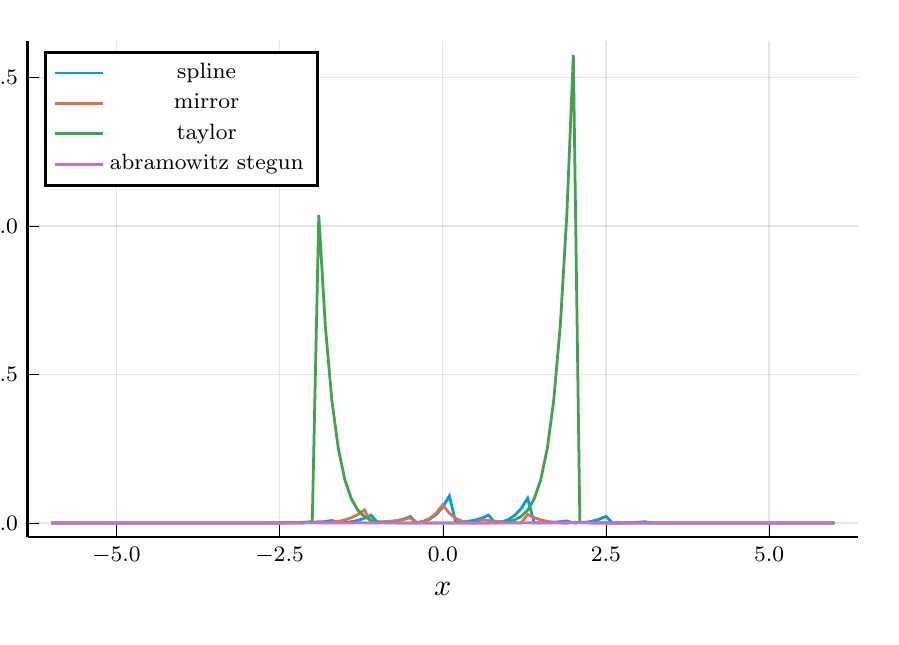
\begin{tikzpicture}[/tikz/background rectangle/.style={fill={rgb,1:red,1.0;green,1.0;blue,1.0}, fill opacity={1.0}, draw opacity={1.0}}, show background rectangle, trim axis left]
\begin{axis}[point meta max={nan}, point meta min={nan}, legend cell align={left}, legend columns={1}, title style={at={{(0.5,1)}}, anchor={south}, font={{\fontsize{14 pt}{18.2 pt}\selectfont}}, color={rgb,1:red,0.0;green,0.0;blue,0.0}, draw opacity={1.0}, rotate={0.0}, align={center}}, legend style={color={rgb,1:red,0.0;green,0.0;blue,0.0}, draw opacity={1.0}, line width={1}, solid, fill={rgb,1:red,1.0;green,1.0;blue,1.0}, fill opacity={1.0}, text opacity={1.0}, font={{\fontsize{8 pt}{10.4 pt}\selectfont}}, text={rgb,1:red,0.0;green,0.0;blue,0.0}, cells={anchor={center}}, at={(0.02, 0.98)}, anchor={north west}}, axis background/.style={fill={rgb,1:red,1.0;green,1.0;blue,1.0}, opacity={1.0}}, anchor={north west}, xshift={1.0mm}, yshift={-1.0mm}, width=\textwidth, height=0.65*\textwidth, scaled x ticks={false}, xlabel={$x$}, x tick style={color={rgb,1:red,0.0;green,0.0;blue,0.0}, opacity={1.0}}, x tick label style={color={rgb,1:red,0.0;green,0.0;blue,0.0}, opacity={1.0}, rotate={0}}, xlabel style={at={(ticklabel cs:0.5)}, anchor=near ticklabel, at={{(ticklabel cs:0.5)}}, anchor={near ticklabel}, font={{\fontsize{11 pt}{14.3 pt}\selectfont}}, color={rgb,1:red,0.0;green,0.0;blue,0.0}, draw opacity={1.0}, rotate={0.0}}, xmajorgrids={true}, xmin={-6.359999799000001}, xmax={6.359993099}, xticklabels={{$-5.0$,$-2.5$,$0.0$,$2.5$,$5.0$}}, xtick={{-5.0,-2.5,0.0,2.5,5.0}}, xtick align={inside}, xticklabel style={font={{\fontsize{8 pt}{10.4 pt}\selectfont}}, color={rgb,1:red,0.0;green,0.0;blue,0.0}, draw opacity={1.0}, rotate={0.0}}, x grid style={color={rgb,1:red,0.0;green,0.0;blue,0.0}, draw opacity={0.1}, line width={0.5}, solid}, axis x line*={left}, x axis line style={color={rgb,1:red,0.0;green,0.0;blue,0.0}, draw opacity={1.0}, line width={1}, solid}, scaled y ticks={false}, ylabel={err}, y tick style={color={rgb,1:red,0.0;green,0.0;blue,0.0}, opacity={1.0}}, y tick label style={color={rgb,1:red,0.0;green,0.0;blue,0.0}, opacity={1.0}, rotate={0}}, ylabel style={at={(ticklabel cs:0.5)}, anchor=near ticklabel, at={{(ticklabel cs:0.5)}}, anchor={near ticklabel}, font={{\fontsize{11 pt}{14.3 pt}\selectfont}}, color={rgb,1:red,0.0;green,0.0;blue,0.0}, draw opacity={1.0}, rotate={0.0}}, ymajorgrids={true}, ymin={-0.04726832820000004}, ymax={1.6228792682000002}, yticklabels={{$0.0$,$0.5$,$1.0$,$1.5$}}, ytick={{0.0,0.5,1.0,1.5}}, ytick align={inside}, yticklabel style={font={{\fontsize{8 pt}{10.4 pt}\selectfont}}, color={rgb,1:red,0.0;green,0.0;blue,0.0}, draw opacity={1.0}, rotate={0.0}}, y grid style={color={rgb,1:red,0.0;green,0.0;blue,0.0}, draw opacity={0.1}, line width={0.5}, solid}, axis y line*={left}, y axis line style={color={rgb,1:red,0.0;green,0.0;blue,0.0}, draw opacity={1.0}, line width={1}, solid}, colorbar={false}]
    \addplot[color={rgb,1:red,0.0;green,0.6056;blue,0.9787}, name path={6}, draw opacity={1.0}, line width={1}, solid]
        table[row sep={\\}]
        {
            \\
            -6.0  0.0  \\
            -5.9  0.0  \\
            -5.8  0.0  \\
            -5.7000003  0.0  \\
            -5.6000004  0.0  \\
            -5.5000005  0.0  \\
            -5.4000006  0.0  \\
            -5.3000007  0.0  \\
            -5.200001  0.0  \\
            -5.100001  0.0  \\
            -5.000001  0.0  \\
            -4.900001  0.0  \\
            -4.800001  0.0  \\
            -4.7000012  0.0  \\
            -4.6000013  0.0  \\
            -4.5000014  0.0  \\
            -4.4000015  0.0  \\
            -4.3000016  0.0  \\
            -4.2000017  0.0  \\
            -4.100002  0.0  \\
            -4.000002  0.0  \\
            -3.900002  5.999999996841865e-8  \\
            -3.800002  5.999999996841865e-8  \\
            -3.7000022  2.0000000000575113e-7  \\
            -3.6000023  3.600000000325565e-7  \\
            -3.5000024  6.999999999646178e-7  \\
            -3.4000025  1.5500000000168157e-6  \\
            -3.3000026  3.0399999999541905e-6  \\
            -3.2000027  5.999999999950489e-6  \\
            -3.1000028  1.1600000000000499e-5  \\
            -3.0000029  2.2100000000024878e-5  \\
            -2.900003  4.10699999999764e-5  \\
            -2.800003  9.730000000041095e-6  \\
            -2.7000031  3.694999999992454e-5  \\
            -2.6000032  9.739000000008602e-5  \\
            -2.5000033  0.00021660000000001123  \\
            -2.4000034  0.0004351000000000216  \\
            -2.3000035  0.0008140600000000608  \\
            -2.2000036  0.00015150000000008212  \\
            -2.1000037  0.0005268499999999676  \\
            -2.0000038  0.0012868000000000324  \\
            -1.9000038  0.002659599999999984  \\
            -1.8000038  0.004955900000000013  \\
            -1.7000037  0.008584139999999962  \\
            -1.6000037  0.00043106000000003863  \\
            -1.5000037  0.0016782699999999817  \\
            -1.4000037  0.004255099999999956  \\
            -1.3000036  0.008779699999999946  \\
            -1.2000036  0.015949559999999918  \\
            -1.1000036  0.02650039999999998  \\
            -1.0000036  0.0009310200000000046  \\
            -0.90000355  0.00228510000000004  \\
            -0.8000035  0.004333840000000033  \\
            -0.7000035  0.007598109999999991  \\
            -0.6000035  0.012923030000000058  \\
            -0.50000346  0.021541450000000018  \\
            -0.40000346  0.000904299999999969  \\
            -0.30000347  0.0046630300000000124  \\
            -0.20000347  0.013175660000000006  \\
            -0.10000347  0.02868522000000001  \\
            -3.4719706e-6  0.0536839536994  \\
            0.09999653  0.09079496  \\
            0.19999653  0.0015377699999999939  \\
            0.29999653  0.003502580000000033  \\
            0.39999652  0.006173450000000025  \\
            0.4999965  0.010173149999999964  \\
            0.5999965  0.016530339999999977  \\
            0.69999653  0.026707640000000032  \\
            0.79999655  0.00018200000000001548  \\
            0.8999966  0.003153650000000008  \\
            0.9999966  0.01077309999999998  \\
            1.0999966  0.025146900000000083  \\
            1.1999966  0.048548399999999936  \\
            1.2999966  0.08333810000000008  \\
            1.3999966  0.00044354999999995925  \\
            1.4999967  0.0009853800000000357  \\
            1.5999967  0.0016796599999999717  \\
            1.6999967  0.0026855999999999547  \\
            1.7999967  0.004278759999999937  \\
            1.8999968  0.006851909999999961  \\
            1.9999968  2.7180000000015525e-5  \\
            2.0999968  0.0008048999999999973  \\
            2.1999967  0.0028256000000000947  \\
            2.2999966  0.006649099999999963  \\
            2.3999965  0.012887749999999976  \\
            2.4999964  0.02219389999999999  \\
            2.5999963  6.430000000001712e-6  \\
            2.6999962  0.0001498499999998959  \\
            2.7999961  0.0005313399999999913  \\
            2.899996  0.0012616000000000849  \\
            2.999996  0.0024583000000000244  \\
            3.0999959  0.004242600000000096  \\
            3.1999958  5.999999999950489e-6  \\
            3.2999957  3.0399999999541905e-6  \\
            3.3999956  1.5500000000168157e-6  \\
            3.4999955  6.999999999646178e-7  \\
            3.5999954  3.600000000325565e-7  \\
            3.6999953  2.0000000000575113e-7  \\
            3.7999952  5.999999996841865e-8  \\
            3.899995  5.999999996841865e-8  \\
            3.999995  0.0  \\
            4.099995  0.0  \\
            4.199995  0.0  \\
            4.299995  0.0  \\
            4.399995  0.0  \\
            4.4999948  0.0  \\
            4.5999947  0.0  \\
            4.6999946  0.0  \\
            4.7999945  0.0  \\
            4.8999944  0.0  \\
            4.9999943  0.0  \\
            5.099994  0.0  \\
            5.199994  0.0  \\
            5.299994  0.0  \\
            5.399994  0.0  \\
            5.499994  0.0  \\
            5.5999937  0.0  \\
            5.6999936  0.0  \\
            5.7999935  0.0  \\
            5.8999934  0.0  \\
            5.9999933  0.0  \\
        }
        ;
    \addlegendentry {spline}
    \addplot[color={rgb,1:red,0.8889;green,0.4356;blue,0.2781}, name path={7}, draw opacity={1.0}, line width={1}, solid]
        table[row sep={\\}]
        {
            \\
            -6.0  0.0  \\
            -5.9  0.0  \\
            -5.8  0.0  \\
            -5.7000003  0.0  \\
            -5.6000004  0.0  \\
            -5.5000005  0.0  \\
            -5.4000006  0.0  \\
            -5.3000007  0.0  \\
            -5.200001  0.0  \\
            -5.100001  0.0  \\
            -5.000001  0.0  \\
            -4.900001  0.0  \\
            -4.800001  0.0  \\
            -4.7000012  0.0  \\
            -4.6000013  0.0  \\
            -4.5000014  0.0  \\
            -4.4000015  0.0  \\
            -4.3000016  0.0  \\
            -4.2000017  0.0  \\
            -4.100002  0.0  \\
            -4.000002  0.0  \\
            -3.900002  5.999999996841865e-8  \\
            -3.800002  5.999999996841865e-8  \\
            -3.7000022  2.0000000000575113e-7  \\
            -3.6000023  3.600000000325565e-7  \\
            -3.5000024  6.999999999646178e-7  \\
            -3.4000025  1.5500000000168157e-6  \\
            -3.3000026  3.0399999999541905e-6  \\
            -3.2000027  1.6000000000016e-5  \\
            -3.1000028  4.009999999998737e-5  \\
            -3.0000029  7.510000000010564e-5  \\
            -2.900003  0.00012527000000006616  \\
            -2.800003  0.0001980000000001425  \\
            -2.7000031  0.00030394999999994177  \\
            -2.6000032  0.00046133000000014857  \\
            -2.5000033  8.559999999935286e-6  \\
            -2.4000034  7.34999999999486e-5  \\
            -2.3000035  0.0002496300000000007  \\
            -2.2000036  0.0006215000000000526  \\
            -2.1000037  0.0013135999999999148  \\
            -2.0000038  0.002503509999999931  \\
            -1.9000038  0.004435560000000005  \\
            -1.8000038  0.0008157300000000145  \\
            -1.7000037  0.0025047599999999948  \\
            -1.6000037  0.005523900000000026  \\
            -1.5000037  0.01044719999999999  \\
            -1.4000037  0.01796544  \\
            -1.3000036  0.028873999999999955  \\
            -1.2000036  0.04404743  \\
            -1.1000036  0.001351250000000026  \\
            -1.0000036  0.0027931700000000115  \\
            -0.90000355  0.004288199999999964  \\
            -0.8000035  0.005965590000000076  \\
            -0.7000035  0.008202970000000032  \\
            -0.6000035  0.011702870000000032  \\
            -0.50000346  0.017555199999999993  \\
            -0.40000346  0.00107024  \\
            -0.30000347  0.0055001300000000475  \\
            -0.20000347  0.01533757999999999  \\
            -0.10000347  0.03297398500000001  \\
            -3.4719706e-6  0.0610501456994  \\
            0.09999653  0.03297556  \\
            0.19999653  0.015338489999999982  \\
            0.29999653  0.005500620000000012  \\
            0.39999652  0.0010704000000000269  \\
            0.4999965  0.0  \\
            0.5999965  0.011703240000000004  \\
            0.69999653  0.008203139999999998  \\
            0.79999655  0.005965740000000053  \\
            0.8999966  0.004288340000000002  \\
            0.9999966  0.00279324000000003  \\
            1.0999966  0.0013513500000000844  \\
            1.1999966  6.999999990764394e-8  \\
            1.2999966  0.028874960000000005  \\
            1.3999966  0.017966069999999945  \\
            1.4999967  0.01044761999999999  \\
            1.5999967  0.005524099999999921  \\
            1.6999967  0.002504900000000032  \\
            1.7999967  0.0008158499999999513  \\
            1.8999968  0.0  \\
            1.9999968  0.002503629999999979  \\
            2.0999968  0.0013136999999999732  \\
            2.1999967  0.0006215000000000526  \\
            2.2999966  0.00024959999999996096  \\
            2.3999965  7.35499999999778e-5  \\
            2.4999964  8.659999999993673e-6  \\
            2.5999963  0.0  \\
            2.6999962  0.00030394999999994177  \\
            2.7999961  0.00019804000000012145  \\
            2.899996  0.00012530000000010588  \\
            2.999996  7.510000000010564e-5  \\
            3.0999959  4.009999999998737e-5  \\
            3.1999958  1.6000000000016e-5  \\
            3.2999957  0.0  \\
            3.3999956  1.5500000000168157e-6  \\
            3.4999955  6.999999999646178e-7  \\
            3.5999954  3.600000000325565e-7  \\
            3.6999953  2.0000000000575113e-7  \\
            3.7999952  5.999999996841865e-8  \\
            3.899995  5.999999996841865e-8  \\
            3.999995  0.0  \\
            4.099995  0.0  \\
            4.199995  0.0  \\
            4.299995  0.0  \\
            4.399995  0.0  \\
            4.4999948  0.0  \\
            4.5999947  0.0  \\
            4.6999946  0.0  \\
            4.7999945  0.0  \\
            4.8999944  0.0  \\
            4.9999943  0.0  \\
            5.099994  0.0  \\
            5.199994  0.0  \\
            5.299994  0.0  \\
            5.399994  0.0  \\
            5.499994  0.0  \\
            5.5999937  0.0  \\
            5.6999936  0.0  \\
            5.7999935  0.0  \\
            5.8999934  0.0  \\
            5.9999933  0.0  \\
        }
        ;
    \addlegendentry {mirror}
    \addplot[color={rgb,1:red,0.2422;green,0.6433;blue,0.3044}, name path={8}, draw opacity={1.0}, line width={1}, solid]
        table[row sep={\\}]
        {
            \\
            -6.0  0.0  \\
            -5.9  0.0  \\
            -5.8  0.0  \\
            -5.7000003  0.0  \\
            -5.6000004  0.0  \\
            -5.5000005  0.0  \\
            -5.4000006  0.0  \\
            -5.3000007  0.0  \\
            -5.200001  0.0  \\
            -5.100001  0.0  \\
            -5.000001  0.0  \\
            -4.900001  0.0  \\
            -4.800001  0.0  \\
            -4.7000012  0.0  \\
            -4.6000013  0.0  \\
            -4.5000014  0.0  \\
            -4.4000015  0.0  \\
            -4.3000016  0.0  \\
            -4.2000017  0.0  \\
            -4.100002  0.0  \\
            -4.000002  0.0  \\
            -3.900002  5.999999996841865e-8  \\
            -3.800002  5.999999996841865e-8  \\
            -3.7000022  2.0000000000575113e-7  \\
            -3.6000023  3.600000000325565e-7  \\
            -3.5000024  6.999999999646178e-7  \\
            -3.4000025  1.5500000000168157e-6  \\
            -3.3000026  3.0399999999541905e-6  \\
            -3.2000027  5.999999999950489e-6  \\
            -3.1000028  1.1600000000000499e-5  \\
            -3.0000029  2.2100000000024878e-5  \\
            -2.900003  4.10699999999764e-5  \\
            -2.800003  7.500000000004725e-5  \\
            -2.7000031  0.0001343499999999498  \\
            -2.6000032  0.0002360300000000537  \\
            -2.5000033  0.0004068999999999878  \\
            -2.4000034  0.0006884999999999808  \\
            -2.3000035  0.001143160000000032  \\
            -2.2000036  0.0018628000000000533  \\
            -2.1000037  0.0029793999999999654  \\
            -2.0000038  0.004677649999999978  \\
            -1.9000038  1.036250575  \\
            -1.8000038  0.6642402000000001  \\
            -1.7000037  0.41374830000000007  \\
            -1.6000037  0.2495522  \\
            -1.5000037  0.14513684999999998  \\
            -1.4000037  0.08098333000000002  \\
            -1.3000036  0.04308776000000003  \\
            -1.2000036  0.02169540000000003  \\
            -1.1000036  0.010240570000000004  \\
            -1.0000036  0.004476429999999976  \\
            -0.90000355  0.0017835600000000174  \\
            -0.8000035  0.0006339000000000761  \\
            -0.7000035  0.00019504000000003519  \\
            -0.6000035  4.970000000004138e-5  \\
            -0.50000346  9.799999999948739e-6  \\
            -0.40000346  1.3500000000110646e-6  \\
            -0.30000347  1.3000000004259604e-7  \\
            -0.20000347  9.999999994736442e-9  \\
            -0.10000347  1.000000000861423e-8  \\
            -3.4719706e-6  3.999999997569316e-13  \\
            0.09999653  5.999999996841865e-9  \\
            0.19999653  9.999999994736442e-9  \\
            0.29999653  1.1999999999234845e-7  \\
            0.39999652  1.360000000005801e-6  \\
            0.4999965  9.849999999977932e-6  \\
            0.5999965  4.97099999999806e-5  \\
            0.69999653  0.0001951000000000036  \\
            0.79999655  0.000633899999999965  \\
            0.8999966  0.0017833999999999905  \\
            0.9999966  0.00447624000000002  \\
            1.0999966  0.01023990000000008  \\
            1.1999966  0.021694369999999963  \\
            1.2999966  0.043085700000000005  \\
            1.3999966  0.08097985000000008  \\
            1.4999967  0.14513115  \\
            1.5999967  0.24954320000000008  \\
            1.6999967  0.41373415999999996  \\
            1.7999967  0.6642188600000001  \\
            1.8999968  1.03621903  \\
            1.9999968  1.57561094  \\
            2.0999968  0.002979500000000024  \\
            2.1999967  0.0018629000000000007  \\
            2.2999966  0.0011432000000000109  \\
            2.3999965  0.00068855000000001  \\
            2.4999964  0.0004070000000000462  \\
            2.5999963  0.0002360300000000537  \\
            2.6999962  0.0001343499999999498  \\
            2.7999961  7.50400000000262e-5  \\
            2.899996  4.1100000000016124e-5  \\
            2.999996  2.2100000000024878e-5  \\
            3.0999959  1.1600000000000499e-5  \\
            3.1999958  5.999999999950489e-6  \\
            3.2999957  3.0399999999541905e-6  \\
            3.3999956  1.5500000000168157e-6  \\
            3.4999955  6.999999999646178e-7  \\
            3.5999954  3.600000000325565e-7  \\
            3.6999953  2.0000000000575113e-7  \\
            3.7999952  5.999999996841865e-8  \\
            3.899995  5.999999996841865e-8  \\
            3.999995  0.0  \\
            4.099995  0.0  \\
            4.199995  0.0  \\
            4.299995  0.0  \\
            4.399995  0.0  \\
            4.4999948  0.0  \\
            4.5999947  0.0  \\
            4.6999946  0.0  \\
            4.7999945  0.0  \\
            4.8999944  0.0  \\
            4.9999943  0.0  \\
            5.099994  0.0  \\
            5.199994  0.0  \\
            5.299994  0.0  \\
            5.399994  0.0  \\
            5.499994  0.0  \\
            5.5999937  0.0  \\
            5.6999936  0.0  \\
            5.7999935  0.0  \\
            5.8999934  0.0  \\
            5.9999933  0.0  \\
        }
        ;
    \addlegendentry {taylor}
    \addplot[color={rgb,1:red,0.7644;green,0.4441;blue,0.8243}, name path={9}, draw opacity={1.0}, line width={1}, solid]
        table[row sep={\\}]
        {
            \\
            -6.0  0.0  \\
            -5.9  0.0  \\
            -5.8  0.0  \\
            -5.7000003  0.0  \\
            -5.6000004  0.0  \\
            -5.5000005  0.0  \\
            -5.4000006  5.999999996841865e-8  \\
            -5.3000007  5.999999996841865e-8  \\
            -5.200001  5.999999996841865e-8  \\
            -5.100001  5.999999996841865e-8  \\
            -5.000001  9.999999994736442e-8  \\
            -4.900001  9.999999994736442e-8  \\
            -4.800001  2.0000000000575113e-7  \\
            -4.7000012  2.399999999846969e-7  \\
            -4.6000013  2.9999999995311555e-7  \\
            -4.5000014  4.0000000001150227e-7  \\
            -4.4000015  6.000000000172534e-7  \\
            -4.3000016  8.299999999517027e-7  \\
            -4.2000017  1.1300000000158406e-6  \\
            -4.100002  1.600000000046009e-6  \\
            -4.000002  2.260000000031681e-6  \\
            -3.900002  3.1000000000336314e-6  \\
            -3.800002  4.439999999994448e-6  \\
            -3.7000022  6.240000000046209e-6  \\
            -3.6000023  8.879999999988897e-6  \\
            -3.5000024  1.2600000000029254e-5  \\
            -3.4000025  1.7750000000038568e-5  \\
            -3.3000026  2.5160000000079563e-5  \\
            -3.2000027  3.5300000000071385e-5  \\
            -3.1000028  4.9300000000029875e-5  \\
            -3.0000029  6.810000000001537e-5  \\
            -2.900003  9.298000000002027e-5  \\
            -2.800003  0.0001250999999999891  \\
            -2.7000031  0.0001651500000000583  \\
            -2.6000032  0.00021350999999991682  \\
            -2.5000033  0.00026890000000001635  \\
            -2.4000034  0.0003283000000000591  \\
            -2.3000035  0.00038629999999995057  \\
            -2.2000036  0.0004345999999999517  \\
            -2.1000037  0.00046204999999999163  \\
            -2.0000038  0.0004561499999999885  \\
            -1.9000038  0.0004049999999999887  \\
            -1.8000038  0.00030160000000001297  \\
            -1.7000037  0.0001476000000000255  \\
            -1.6000037  4.170000000003338e-5  \\
            -1.5000037  0.0002358999999999556  \\
            -1.4000037  0.00039226999999997236  \\
            -1.3000036  0.00046464000000001615  \\
            -1.2000036  0.0004185999999999357  \\
            -1.1000036  0.00024884000000002793  \\
            -1.0000036  8.110000000005613e-6  \\
            -0.90000355  0.0002733999999999792  \\
            -0.8000035  0.0004445400000000488  \\
            -0.7000035  0.00043440000000005696  \\
            -0.6000035  0.00021850000000001035  \\
            -0.50000346  0.00012500000000004174  \\
            -0.40000346  0.00041322999999998666  \\
            -0.30000347  0.00042436999999995173  \\
            -0.20000347  5.288999999999988e-5  \\
            -0.10000347  0.00042556500000000275  \\
            -3.4719706e-6  1.0300210000000011e-7  \\
            0.09999653  0.00042560999999999294  \\
            0.19999653  5.28000000000195e-5  \\
            0.29999653  0.000424380000000002  \\
            0.39999652  0.00041330000000000533  \\
            0.4999965  0.0001249899999999915  \\
            0.5999965  0.0002185100000000606  \\
            0.69999653  0.0004343300000000383  \\
            0.79999655  0.0004444999999999588  \\
            0.8999966  0.0002733999999999792  \\
            0.9999966  8.160000000034806e-6  \\
            1.0999966  0.00024879999999993796  \\
            1.1999966  0.00041863000000008643  \\
            1.2999966  0.0004646499999999554  \\
            1.3999966  0.0003922299999999934  \\
            1.4999967  0.00023591000000000584  \\
            1.5999967  4.1699999999922355e-5  \\
            1.6999967  0.0001476000000000255  \\
            1.7999967  0.00030160000000001297  \\
            1.8999968  0.00040507000000000737  \\
            1.9999968  0.0004560700000000306  \\
            2.0999968  0.00046210000000002083  \\
            2.1999967  0.00043455999999997275  \\
            2.2999966  0.00038629999999995057  \\
            2.3999965  0.0003282500000000299  \\
            2.4999964  0.00026879999999995796  \\
            2.5999963  0.00021350999999991682  \\
            2.6999962  0.0001651500000000583  \\
            2.7999961  0.00012506000000001016  \\
            2.899996  9.300000000000974e-5  \\
            2.999996  6.810000000001537e-5  \\
            3.0999959  4.9300000000029875e-5  \\
            3.1999958  3.5300000000071385e-5  \\
            3.2999957  2.5160000000079563e-5  \\
            3.3999956  1.7750000000038568e-5  \\
            3.4999955  1.2600000000029254e-5  \\
            3.5999954  8.879999999988897e-6  \\
            3.6999953  6.240000000046209e-6  \\
            3.7999952  4.439999999994448e-6  \\
            3.899995  3.1000000000336314e-6  \\
            3.999995  2.260000000031681e-6  \\
            4.099995  1.600000000046009e-6  \\
            4.199995  1.1300000000158406e-6  \\
            4.299995  8.299999999517027e-7  \\
            4.399995  6.000000000172534e-7  \\
            4.4999948  4.0000000001150227e-7  \\
            4.5999947  2.9999999995311555e-7  \\
            4.6999946  2.399999999846969e-7  \\
            4.7999945  2.0000000000575113e-7  \\
            4.8999944  9.999999994736442e-8  \\
            4.9999943  9.999999994736442e-8  \\
            5.099994  5.999999996841865e-8  \\
            5.199994  5.999999996841865e-8  \\
            5.299994  5.999999996841865e-8  \\
            5.399994  5.999999996841865e-8  \\
            5.499994  0.0  \\
            5.5999937  0.0  \\
            5.6999936  0.0  \\
            5.7999935  0.0  \\
            5.8999934  0.0  \\
            5.9999933  0.0  \\
        }
        ;
    \addlegendentry {abramowitz stegun}
\end{axis}
\end{tikzpicture}

        \caption{$\erf$ Errors}
    \end{figure}
    
    \begin{figure}[h]
        \centering
        % Recommended preamble:
% \usetikzlibrary{arrows.meta}
% \usetikzlibrary{backgrounds}
% \usepgfplotslibrary{patchplots}
% \usepgfplotslibrary{fillbetween}
% \pgfplotsset{%
%     layers/standard/.define layer set={%
%         background,axis background,axis grid,axis ticks,axis lines,axis tick labels,pre main,main,axis descriptions,axis foreground%
%     }{
%         grid style={/pgfplots/on layer=axis grid},%
%         tick style={/pgfplots/on layer=axis ticks},%
%         axis line style={/pgfplots/on layer=axis lines},%
%         label style={/pgfplots/on layer=axis descriptions},%
%         legend style={/pgfplots/on layer=axis descriptions},%
%         title style={/pgfplots/on layer=axis descriptions},%
%         colorbar style={/pgfplots/on layer=axis descriptions},%
%         ticklabel style={/pgfplots/on layer=axis tick labels},%
%         axis background@ style={/pgfplots/on layer=axis background},%
%         3d box foreground style={/pgfplots/on layer=axis foreground},%
%     },
% }

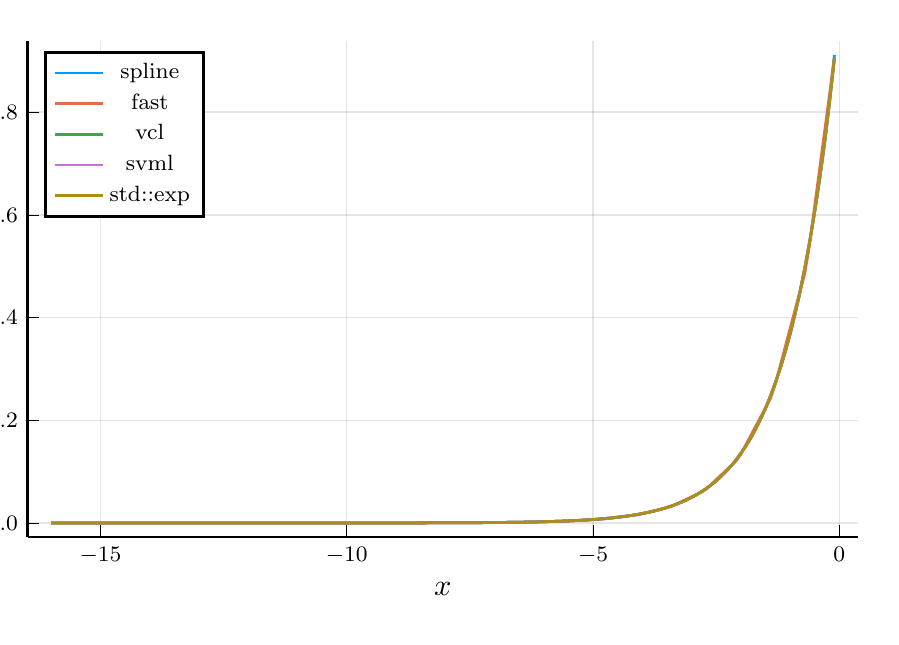
\begin{tikzpicture}[/tikz/background rectangle/.style={fill={rgb,1:red,1.0;green,1.0;blue,1.0}, fill opacity={1.0}, draw opacity={1.0}}, show background rectangle, trim axis left]
\begin{axis}[point meta max={nan}, point meta min={nan}, legend cell align={left}, legend columns={1}, title={}, title style={at={{(0.5,1)}}, anchor={south}, font={{\fontsize{14 pt}{18.2 pt}\selectfont}}, color={rgb,1:red,0.0;green,0.0;blue,0.0}, draw opacity={1.0}, rotate={0.0}, align={center}}, legend style={color={rgb,1:red,0.0;green,0.0;blue,0.0}, draw opacity={1.0}, line width={1}, solid, fill={rgb,1:red,1.0;green,1.0;blue,1.0}, fill opacity={1.0}, text opacity={1.0}, font={{\fontsize{8 pt}{10.4 pt}\selectfont}}, text={rgb,1:red,0.0;green,0.0;blue,0.0}, cells={anchor={center}}, at={(0.02, 0.98)}, anchor={north west}}, axis background/.style={fill={rgb,1:red,1.0;green,1.0;blue,1.0}, opacity={1.0}}, anchor={north west}, xshift={1.0mm}, yshift={-1.0mm}, width=\textwidth, height=0.65*\textwidth, scaled x ticks={false}, xlabel={$x$}, x tick style={color={rgb,1:red,0.0;green,0.0;blue,0.0}, opacity={1.0}}, x tick label style={color={rgb,1:red,0.0;green,0.0;blue,0.0}, opacity={1.0}, rotate={0}}, xlabel style={at={(ticklabel cs:0.5)}, anchor=near ticklabel, at={{(ticklabel cs:0.5)}}, anchor={near ticklabel}, font={{\fontsize{11 pt}{14.3 pt}\selectfont}}, color={rgb,1:red,0.0;green,0.0;blue,0.0}, draw opacity={1.0}, rotate={0.0}}, xmajorgrids={true}, xmin={-16.4770000357}, xmax={0.37700122570000083}, xticklabels={{$-15$,$-10$,$-5$,$0$}}, xtick={{-15.0,-10.0,-5.0,0.0}}, xtick align={inside}, xticklabel style={font={{\fontsize{8 pt}{10.4 pt}\selectfont}}, color={rgb,1:red,0.0;green,0.0;blue,0.0}, draw opacity={1.0}, rotate={0.0}}, x grid style={color={rgb,1:red,0.0;green,0.0;blue,0.0}, draw opacity={0.1}, line width={0.5}, solid}, axis x line*={left}, x axis line style={color={rgb,1:red,0.0;green,0.0;blue,0.0}, draw opacity={1.0}, line width={1}, solid}, scaled y ticks={false}, ylabel={$y$}, y tick style={color={rgb,1:red,0.0;green,0.0;blue,0.0}, opacity={1.0}}, y tick label style={color={rgb,1:red,0.0;green,0.0;blue,0.0}, opacity={1.0}, rotate={0}}, ylabel style={at={(ticklabel cs:0.5)}, anchor=near ticklabel, at={{(ticklabel cs:0.5)}}, anchor={near ticklabel}, font={{\fontsize{11 pt}{14.3 pt}\selectfont}}, color={rgb,1:red,0.0;green,0.0;blue,0.0}, draw opacity={1.0}, rotate={0.0}}, ymajorgrids={true}, ymin={-0.027340977000000044}, ymax={0.938706877}, yticklabels={{$0.0$,$0.2$,$0.4$,$0.6$,$0.8$}}, ytick={{0.0,0.2,0.4,0.6000000000000001,0.8}}, ytick align={inside}, yticklabel style={font={{\fontsize{8 pt}{10.4 pt}\selectfont}}, color={rgb,1:red,0.0;green,0.0;blue,0.0}, draw opacity={1.0}, rotate={0.0}}, y grid style={color={rgb,1:red,0.0;green,0.0;blue,0.0}, draw opacity={0.1}, line width={0.5}, solid}, axis y line*={left}, y axis line style={color={rgb,1:red,0.0;green,0.0;blue,0.0}, draw opacity={1.0}, line width={1}, solid}, colorbar={false}]
    \addplot[color={rgb,1:red,0.0;green,0.6056;blue,0.9787}, name path={12}, draw opacity={1.0}, line width={1}, solid]
        table[row sep={\\}]
        {
            \\
            -16.0  0.0  \\
            -15.9  0.0  \\
            -15.8  0.0  \\
            -15.7  0.0  \\
            -15.6  0.0  \\
            -15.5  0.0  \\
            -15.4  0.0  \\
            -15.3  0.0  \\
            -15.2  0.0  \\
            -15.1  0.0  \\
            -15.0  0.0  \\
            -14.9  0.0  \\
            -14.8  0.0  \\
            -14.7  0.0  \\
            -14.6  0.0  \\
            -14.5  0.0  \\
            -14.4  0.0  \\
            -14.299999  0.0  \\
            -14.2  0.0  \\
            -14.099999  0.0  \\
            -14.0  0.0  \\
            -13.9  0.0  \\
            -13.799999  0.0  \\
            -13.7  0.0  \\
            -13.599999  0.0  \\
            -13.5  0.0  \\
            -13.4  0.0  \\
            -13.299999  0.0  \\
            -13.2  0.0  \\
            -13.099999  0.0  \\
            -13.0  0.0  \\
            -12.9  0.0  \\
            -12.799999  0.0  \\
            -12.699999  0.0  \\
            -12.599999  0.0  \\
            -12.499999  0.0  \\
            -12.4  0.0  \\
            -12.299999  0.0  \\
            -12.199999  0.0  \\
            -12.099999  0.0  \\
            -11.999999  0.0  \\
            -11.9  0.0  \\
            -11.799999  0.0  \\
            -11.699999  0.0  \\
            -11.599999  0.0  \\
            -11.499999  0.0  \\
            -11.4  0.0  \\
            -11.299999  0.0  \\
            -11.199999  0.0  \\
            -11.099998  0.0  \\
            -10.999999  0.0  \\
            -10.899999  0.0  \\
            -10.799999  0.0  \\
            -10.699999  0.0  \\
            -10.599998  0.0  \\
            -10.499999  0.0  \\
            -10.399999  0.0  \\
            -10.299999  0.0  \\
            -10.199999  0.0  \\
            -10.099998  0.0  \\
            -9.999999  0.0  \\
            -9.899999  0.0  \\
            -9.799999  0.0  \\
            -9.699999  0.0  \\
            -9.599998  0.0  \\
            -9.499998  0.0  \\
            -9.399999  0.0  \\
            -9.299998  0.0  \\
            -9.199999  0.0  \\
            -9.099998  0.0  \\
            -8.999998  0.00012341003  \\
            -8.899999  0.00013604923  \\
            -8.799998  0.00015007092  \\
            -8.699999  0.00016560049  \\
            -8.599998  0.00018276392  \\
            -8.499998  0.00020168674  \\
            -8.399999  0.0002224944  \\
            -8.299998  0.000245313  \\
            -8.199999  0.0002702677  \\
            -8.099998  0.00029748472  \\
            -7.9999986  0.0003354631  \\
            -7.8999987  0.0003703528  \\
            -7.7999988  0.00040843422  \\
            -7.6999984  0.00044988346  \\
            -7.5999985  0.00049487606  \\
            -7.4999986  0.00054358813  \\
            -7.3999987  0.0005961955  \\
            -7.2999988  0.00065287424  \\
            -7.1999984  0.00071380043  \\
            -7.0999985  0.00077914936  \\
            -6.9999986  0.00091188325  \\
            -6.8999987  0.0010073882  \\
            -6.7999988  0.001111988  \\
            -6.6999984  0.0012262354  \\
            -6.5999985  0.0013506825  \\
            -6.4999986  0.001485882  \\
            -6.3999987  0.0016323866  \\
            -6.2999988  0.001790749  \\
            -6.199999  0.0019615218  \\
            -6.0999985  0.0021452587  \\
            -5.9999986  0.0024787558  \\
            -5.8999987  0.0027351729  \\
            -5.7999988  0.003015203  \\
            -5.699999  0.0033202162  \\
            -5.5999985  0.0036515843  \\
            -5.4999986  0.004010674  \\
            -5.3999987  0.0043988577  \\
            -5.2999988  0.0048175044  \\
            -5.199999  0.0052679847  \\
            -5.0999985  0.0057516713  \\
            -4.9999986  0.006737957  \\
            -4.8999987  0.007447075  \\
            -4.7999988  0.008224397  \\
            -4.699999  0.009074101  \\
            -4.599999  0.010000366  \\
            -4.4999986  0.011109012  \\
            -4.3999987  0.012274925  \\
            -4.2999988  0.013559204  \\
            -4.199999  0.014970906  \\
            -4.099999  0.01651909  \\
            -3.9999988  0.018315662  \\
            -3.8999987  0.020238852  \\
            -3.7999988  0.02235531  \\
            -3.6999989  0.024679031  \\
            -3.5999987  0.027224017  \\
            -3.4999988  0.03019742  \\
            -3.3999987  0.03336753  \\
            -3.2999988  0.036856506  \\
            -3.1999989  0.040687617  \\
            -3.099999  0.04488413  \\
            -2.9999988  0.049787126  \\
            -2.899999  0.0550156  \\
            -2.7999988  0.06077082  \\
            -2.6999989  0.06709127  \\
            -2.599999  0.07401548  \\
            -2.4999988  0.082085095  \\
            -2.399999  0.09069865  \\
            -2.2999988  0.10017645  \\
            -2.1999989  0.11058111  \\
            -2.099999  0.12197532  \\
            -1.9999988  0.13533545  \\
            -1.8999988  0.14956193  \\
            -1.7999989  0.16522908  \\
            -1.6999989  0.1826818  \\
            -1.5999988  0.20187654  \\
            -1.4999988  0.22313043  \\
            -1.3999988  0.24658069  \\
            -1.2999989  0.272439  \\
            -1.1999989  0.3011984  \\
            -1.0999988  0.33286276  \\
            -0.9999988  0.3678799  \\
            -0.89999884  0.4064839  \\
            -0.7999988  0.44899392  \\
            -0.6999988  0.496676  \\
            -0.59999883  0.5492181  \\
            -0.4999988  0.6065314  \\
            -0.3999988  0.6693561  \\
            -0.29999882  0.73767203  \\
            -0.19999881  0.82004696  \\
            -0.09999881  0.9113659  \\
        }
        ;
    \addlegendentry {spline}
    \addplot[color={rgb,1:red,0.8889;green,0.4356;blue,0.2781}, name path={13}, draw opacity={1.0}, line width={1}, solid]
        table[row sep={\\}]
        {
            \\
            -16.0  1.1165139e-7  \\
            -15.9  1.2129203e-7  \\
            -15.8  1.3849058e-7  \\
            -15.7  1.5568821e-7  \\
            -15.6  1.7288676e-7  \\
            -15.5  1.900853e-7  \\
            -15.4  2.0728294e-7  \\
            -15.3  2.2448148e-7  \\
            -15.2  2.4494148e-7  \\
            -15.1  2.7933675e-7  \\
            -15.0  3.1373384e-7  \\
            -14.9  3.4813092e-7  \\
            -14.8  3.8252801e-7  \\
            -14.7  4.1692329e-7  \\
            -14.6  4.5132037e-7  \\
            -14.5  4.9459777e-7  \\
            -14.4  5.633883e-7  \\
            -14.299999  6.321825e-7  \\
            -14.2  7.0097667e-7  \\
            -14.099999  7.6977085e-7  \\
            -14.0  8.385614e-7  \\
            -13.9  9.0735557e-7  \\
            -13.799999  9.986252e-7  \\
            -13.7  1.1362063e-6  \\
            -13.599999  1.2737946e-6  \\
            -13.5  1.411383e-6  \\
            -13.4  1.5489641e-6  \\
            -13.299999  1.6865524e-6  \\
            -13.2  1.8241408e-6  \\
            -13.099999  2.016095e-6  \\
            -13.0  2.2912718e-6  \\
            -12.9  2.5664485e-6  \\
            -12.799999  2.8416252e-6  \\
            -12.699999  3.1167874e-6  \\
            -12.599999  3.3919641e-6  \\
            -12.499999  3.6671408e-6  \\
            -12.4  4.0699088e-6  \\
            -12.299999  4.620262e-6  \\
            -12.199999  5.1706156e-6  \\
            -12.099999  5.72094e-6  \\
            -11.999999  6.2712934e-6  \\
            -11.9  6.821647e-6  \\
            -11.799999  7.371971e-6  \\
            -11.699999  8.215255e-6  \\
            -11.599999  9.3159615e-6  \\
            -11.499999  1.0416668e-5  \\
            -11.4  1.1517317e-5  \\
            -11.299999  1.2618024e-5  \\
            -11.199999  1.3718731e-5  \\
            -11.099998  1.4819379e-5  \\
            -10.999999  1.6581384e-5  \\
            -10.899999  1.8782797e-5  \\
            -10.799999  2.0984095e-5  \\
            -10.699999  2.3185508e-5  \\
            -10.599998  2.5386922e-5  \\
            -10.499999  2.7588336e-5  \\
            -10.399999  2.9789633e-5  \\
            -10.299999  3.3464516e-5  \\
            -10.199999  3.7867343e-5  \\
            -10.099998  4.2269938e-5  \\
            -9.999999  4.6672765e-5  \\
            -9.899999  5.1075593e-5  \\
            -9.799999  5.5478187e-5  \\
            -9.699999  5.9881015e-5  \\
            -9.599998  6.753253e-5  \\
            -9.499998  7.633818e-5  \\
            -9.399999  8.514337e-5  \\
            -9.299998  9.394903e-5  \\
            -9.199999  0.00010275468  \\
            -9.099998  0.00011155987  \\
            -8.999998  0.00012036553  \\
            -8.899999  0.00013627205  \\
            -8.799998  0.00015388243  \\
            -8.699999  0.00017149374  \\
            -8.599998  0.00018910505  \\
            -8.499998  0.00020671636  \\
            -8.399999  0.00022432674  \\
            -8.299998  0.00024193805  \\
            -8.199999  0.00027495623  \\
            -8.099998  0.00031017885  \\
            -7.9999986  0.00034540147  \\
            -7.8999987  0.0003806241  \\
            -7.7999988  0.00041584484  \\
            -7.6999984  0.00045106746  \\
            -7.5999985  0.00048629008  \\
            -7.4999986  0.0005547404  \\
            -7.3999987  0.00062518567  \\
            -7.2999988  0.0006956309  \\
            -7.1999984  0.0007660724  \\
            -7.0999985  0.00083651766  \\
            -6.9999986  0.0009069629  \\
            -6.8999987  0.0009782463  \\
            -6.7999988  0.0011191368  \\
            -6.6999984  0.0012600273  \\
            -6.5999985  0.0014009178  \\
            -6.4999986  0.0015418008  \\
            -6.3999987  0.0016826913  \\
            -6.2999988  0.0018235818  \\
            -6.199999  0.0019758046  \\
            -6.0999985  0.0022575855  \\
            -5.9999986  0.0025393665  \\
            -5.8999987  0.0028211325  \\
            -5.7999988  0.0031029135  \\
            -5.699999  0.0033846945  \\
            -5.5999985  0.0036664754  \\
            -5.4999986  0.003990233  \\
            -5.3999987  0.004553795  \\
            -5.2999988  0.005117357  \\
            -5.199999  0.005680889  \\
            -5.0999985  0.006244451  \\
            -4.9999986  0.0068080127  \\
            -4.8999987  0.007371545  \\
            -4.7999988  0.0080577135  \\
            -4.699999  0.009184837  \\
            -4.599999  0.010311902  \\
            -4.4999986  0.011439025  \\
            -4.3999987  0.012566149  \\
            -4.2999988  0.013693213  \\
            -4.199999  0.014820337  \\
            -4.099999  0.016269922  \\
            -3.9999988  0.01852417  \\
            -3.8999987  0.020778298  \\
            -3.7999988  0.023032546  \\
            -3.6999989  0.025286794  \\
            -3.5999987  0.027540922  \\
            -3.4999988  0.02979517  \\
            -3.3999987  0.032848835  \\
            -3.2999988  0.037357092  \\
            -3.1999989  0.041865587  \\
            -3.099999  0.046374083  \\
            -2.9999988  0.05088234  \\
            -2.899999  0.055390835  \\
            -2.7999988  0.05989933  \\
            -2.6999989  0.06631565  \\
            -2.599999  0.075332165  \\
            -2.4999988  0.084349155  \\
            -2.399999  0.093366146  \\
            -2.2999988  0.10238266  \\
            -2.1999989  0.11139965  \\
            -2.099999  0.12041664  \\
            -1.9999988  0.13386631  \\
            -1.8999988  0.15190029  \\
            -1.7999989  0.16993427  \\
            -1.6999989  0.1879673  \\
            -1.5999988  0.20600128  \\
            -1.4999988  0.22403526  \\
            -1.3999988  0.24206924  \\
            -1.2999989  0.27020454  \\
            -1.1999989  0.3062725  \\
            -1.0999988  0.34234047  \\
            -0.9999988  0.37840652  \\
            -0.89999884  0.4144745  \\
            -0.7999988  0.45054245  \\
            -0.6999988  0.4866085  \\
            -0.59999883  0.54535294  \\
            -0.4999988  0.61748886  \\
            -0.3999988  0.689621  \\
            -0.29999882  0.7617569  \\
            -0.19999881  0.8338928  \\
            -0.09999881  0.90602875  \\
        }
        ;
    \addlegendentry {fast}
    \addplot[color={rgb,1:red,0.2422;green,0.6433;blue,0.3044}, name path={14}, draw opacity={1.0}, line width={1}, solid]
        table[row sep={\\}]
        {
            \\
            -16.0  1.12535176e-7  \\
            -15.9  1.2437064e-7  \\
            -15.8  1.3745074e-7  \\
            -15.7  1.5190662e-7  \\
            -15.6  1.6788269e-7  \\
            -15.5  1.8553914e-7  \\
            -15.4  2.0505254e-7  \\
            -15.3  2.2661797e-7  \\
            -15.2  2.5045168e-7  \\
            -15.1  2.7679175e-7  \\
            -15.0  3.0590232e-7  \\
            -14.9  3.3807447e-7  \\
            -14.8  3.7362986e-7  \\
            -14.7  4.1292503e-7  \\
            -14.6  4.5635247e-7  \\
            -14.5  5.0434767e-7  \\
            -14.4  5.573906e-7  \\
            -14.299999  6.1601213e-7  \\
            -14.2  6.807983e-7  \\
            -14.099999  7.523987e-7  \\
            -14.0  8.315287e-7  \\
            -13.9  9.189817e-7  \\
            -13.799999  1.0156323e-6  \\
            -13.7  1.1224465e-6  \\
            -13.599999  1.2404957e-6  \\
            -13.5  1.3709591e-6  \\
            -13.4  1.5151447e-6  \\
            -13.299999  1.6744945e-6  \\
            -13.2  1.8506015e-6  \\
            -13.099999  2.045232e-6  \\
            -13.0  2.2603294e-6  \\
            -12.9  2.4980513e-6  \\
            -12.799999  2.7607748e-6  \\
            -12.699999  3.0511292e-6  \\
            -12.599999  3.372017e-6  \\
            -12.499999  3.7266568e-6  \\
            -12.4  4.1185904e-6  \\
            -12.299999  4.551748e-6  \\
            -12.199999  5.0304616e-6  \\
            -12.099999  5.5595165e-6  \\
            -11.999999  6.1442183e-6  \\
            -11.9  6.7904075e-6  \\
            -11.799999  7.5045637e-6  \\
            -11.699999  8.293829e-6  \\
            -11.599999  9.166093e-6  \\
            -11.499999  1.0130103e-5  \\
            -11.4  1.1195489e-5  \\
            -11.299999  1.2372933e-5  \\
            -11.199999  1.3674212e-5  \\
            -11.099998  1.5112347e-5  \\
            -10.999999  1.6701717e-5  \\
            -10.899999  1.8458259e-5  \\
            -10.799999  2.0399519e-5  \\
            -10.699999  2.2544964e-5  \\
            -10.599998  2.4916048e-5  \\
            -10.499999  2.7536476e-5  \\
            -10.399999  3.0432524e-5  \\
            -10.299999  3.363312e-5  \\
            -10.199999  3.717036e-5  \\
            -10.099998  4.107962e-5  \\
            -9.999999  4.5399975e-5  \\
            -9.899999  5.017475e-5  \\
            -9.799999  5.545164e-5  \\
            -9.699999  6.1283565e-5  \\
            -9.599998  6.772884e-5  \\
            -9.499998  7.4851974e-5  \\
            -9.399999  8.2724175e-5  \\
            -9.299998  9.142439e-5  \\
            -9.199999  0.00010103952  \\
            -9.099998  0.00011166598  \\
            -8.999998  0.00012341003  \\
            -8.899999  0.0001363891  \\
            -8.799998  0.00015073334  \\
            -8.699999  0.000166586  \\
            -8.599998  0.00018410607  \\
            -8.499998  0.00020346875  \\
            -8.399999  0.00022486763  \\
            -8.299998  0.00024851726  \\
            -8.199999  0.0002746539  \\
            -8.099998  0.0003035396  \\
            -7.9999986  0.0003354631  \\
            -7.8999987  0.00037074403  \\
            -7.7999988  0.00040973548  \\
            -7.6999984  0.00045282792  \\
            -7.5999985  0.0005004522  \\
            -7.4999986  0.0005530852  \\
            -7.3999987  0.00061125355  \\
            -7.2999988  0.0006755396  \\
            -7.1999984  0.000746587  \\
            -7.0999985  0.00082510617  \\
            -6.9999986  0.00091188325  \\
            -6.8999987  0.0010077867  \\
            -6.7999988  0.0011137766  \\
            -6.6999984  0.0012309139  \\
            -6.5999985  0.0013603701  \\
            -6.4999986  0.0015034412  \\
            -6.3999987  0.0016615596  \\
            -6.2999988  0.001836307  \\
            -6.199999  0.002029433  \\
            -6.0999985  0.002242871  \\
            -5.9999986  0.0024787558  \\
            -5.8999987  0.0027394486  \\
            -5.7999988  0.0030275583  \\
            -5.699999  0.0033459694  \\
            -5.5999985  0.0036978694  \\
            -5.4999986  0.004086777  \\
            -5.3999987  0.004516587  \\
            -5.2999988  0.0049916003  \\
            -5.199999  0.0055165705  \\
            -5.0999985  0.006096756  \\
            -4.9999986  0.006737957  \\
            -4.8999987  0.007446593  \\
            -4.7999988  0.008229758  \\
            -4.699999  0.009095288  \\
            -4.599999  0.0100518465  \\
            -4.4999986  0.011109013  \\
            -4.3999987  0.012277356  \\
            -4.2999988  0.0135685755  \\
            -4.199999  0.014995594  \\
            -4.099999  0.016572693  \\
            -3.9999988  0.018315662  \\
            -3.8999987  0.020241939  \\
            -3.7999988  0.0223708  \\
            -3.6999989  0.024723554  \\
            -3.5999987  0.027323756  \\
            -3.4999988  0.03019742  \\
            -3.3999987  0.033373315  \\
            -3.2999988  0.036883213  \\
            -3.1999989  0.040762253  \\
            -3.099999  0.04504925  \\
            -2.9999988  0.049787126  \\
            -2.899999  0.05502328  \\
            -2.7999988  0.060810138  \\
            -2.6999989  0.06720559  \\
            -2.599999  0.07427365  \\
            -2.4999988  0.082085095  \\
            -2.399999  0.09071805  \\
            -2.2999988  0.10025897  \\
            -2.1999989  0.110803284  \\
            -2.099999  0.12245656  \\
            -1.9999988  0.13533545  \\
            -1.8999988  0.1495688  \\
            -1.7999989  0.16529907  \\
            -1.6999989  0.18268374  \\
            -1.5999988  0.20189676  \\
            -1.4999988  0.22313042  \\
            -1.3999988  0.24659726  \\
            -1.2999989  0.2725321  \\
            -1.1999989  0.30119455  \\
            -1.0999988  0.33287147  \\
            -0.9999988  0.36787987  \\
            -0.89999884  0.40657014  \\
            -0.7999988  0.4493295  \\
            -0.6999988  0.4965859  \\
            -0.59999883  0.54881227  \\
            -0.4999988  0.6065314  \\
            -0.3999988  0.67032087  \\
            -0.29999882  0.7408191  \\
            -0.19999881  0.8187317  \\
            -0.09999881  0.9048385  \\
        }
        ;
    \addlegendentry {vcl}
    \addplot[color={rgb,1:red,0.7644;green,0.4441;blue,0.8243}, name path={15}, draw opacity={1.0}, line width={1}, solid]
        table[row sep={\\}]
        {
            \\
            -16.0  1.12535176e-7  \\
            -15.9  1.2437064e-7  \\
            -15.8  1.3745074e-7  \\
            -15.7  1.5190663e-7  \\
            -15.6  1.6788267e-7  \\
            -15.5  1.8553915e-7  \\
            -15.4  2.0505252e-7  \\
            -15.3  2.2661797e-7  \\
            -15.2  2.5045168e-7  \\
            -15.1  2.7679175e-7  \\
            -15.0  3.0590235e-7  \\
            -14.9  3.3807444e-7  \\
            -14.8  3.736299e-7  \\
            -14.7  4.12925e-7  \\
            -14.6  4.5635247e-7  \\
            -14.5  5.0434767e-7  \\
            -14.4  5.573906e-7  \\
            -14.299999  6.160122e-7  \\
            -14.2  6.807982e-7  \\
            -14.099999  7.5239876e-7  \\
            -14.0  8.3152867e-7  \\
            -13.9  9.189817e-7  \\
            -13.799999  1.0156323e-6  \\
            -13.7  1.1224465e-6  \\
            -13.599999  1.240496e-6  \\
            -13.5  1.3709591e-6  \\
            -13.4  1.5151447e-6  \\
            -13.299999  1.6744945e-6  \\
            -13.2  1.8506015e-6  \\
            -13.099999  2.0452317e-6  \\
            -13.0  2.2603294e-6  \\
            -12.9  2.4980516e-6  \\
            -12.799999  2.7607748e-6  \\
            -12.699999  3.0511292e-6  \\
            -12.599999  3.3720169e-6  \\
            -12.499999  3.7266568e-6  \\
            -12.4  4.11859e-6  \\
            -12.299999  4.5517477e-6  \\
            -12.199999  5.030462e-6  \\
            -12.099999  5.559517e-6  \\
            -11.999999  6.1442183e-6  \\
            -11.9  6.790407e-6  \\
            -11.799999  7.5045637e-6  \\
            -11.699999  8.293829e-6  \\
            -11.599999  9.166093e-6  \\
            -11.499999  1.0130105e-5  \\
            -11.4  1.11954905e-5  \\
            -11.299999  1.2372933e-5  \\
            -11.199999  1.3674211e-5  \\
            -11.099998  1.5112347e-5  \\
            -10.999999  1.6701717e-5  \\
            -10.899999  1.8458259e-5  \\
            -10.799999  2.039952e-5  \\
            -10.699999  2.2544966e-5  \\
            -10.599998  2.4916048e-5  \\
            -10.499999  2.7536475e-5  \\
            -10.399999  3.0432524e-5  \\
            -10.299999  3.3633118e-5  \\
            -10.199999  3.717036e-5  \\
            -10.099998  4.1079624e-5  \\
            -9.999999  4.539998e-5  \\
            -9.899999  5.017475e-5  \\
            -9.799999  5.545164e-5  \\
            -9.699999  6.1283565e-5  \\
            -9.599998  6.772883e-5  \\
            -9.499998  7.4851974e-5  \\
            -9.399999  8.272418e-5  \\
            -9.299998  9.14244e-5  \\
            -9.199999  0.00010103951  \\
            -9.099998  0.00011166598  \\
            -8.999998  0.00012341003  \\
            -8.899999  0.0001363891  \\
            -8.799998  0.00015073334  \\
            -8.699999  0.00016658602  \\
            -8.599998  0.00018410609  \\
            -8.499998  0.00020346875  \\
            -8.399999  0.00022486762  \\
            -8.299998  0.00024851726  \\
            -8.199999  0.00027465387  \\
            -8.099998  0.00030353962  \\
            -7.9999986  0.00033546312  \\
            -7.8999987  0.00037074406  \\
            -7.7999988  0.00040973548  \\
            -7.6999984  0.0004528279  \\
            -7.5999985  0.0005004522  \\
            -7.4999986  0.0005530851  \\
            -7.3999987  0.0006112536  \\
            -7.2999988  0.0006755396  \\
            -7.1999984  0.00074658706  \\
            -7.0999985  0.00082510617  \\
            -6.9999986  0.00091188325  \\
            -6.8999987  0.0010077867  \\
            -6.7999988  0.0011137765  \\
            -6.6999984  0.001230914  \\
            -6.5999985  0.0013603701  \\
            -6.4999986  0.0015034415  \\
            -6.3999987  0.0016615595  \\
            -6.2999988  0.001836307  \\
            -6.199999  0.002029433  \\
            -6.0999985  0.002242871  \\
            -5.9999986  0.002478756  \\
            -5.8999987  0.0027394483  \\
            -5.7999988  0.0030275586  \\
            -5.699999  0.0033459691  \\
            -5.5999985  0.0036978694  \\
            -5.4999986  0.004086777  \\
            -5.3999987  0.0045165867  \\
            -5.2999988  0.0049916008  \\
            -5.199999  0.00551657  \\
            -5.0999985  0.006096756  \\
            -4.9999986  0.0067379563  \\
            -4.8999987  0.007446593  \\
            -4.7999988  0.008229757  \\
            -4.699999  0.009095287  \\
            -4.599999  0.010051847  \\
            -4.4999986  0.011109011  \\
            -4.3999987  0.012277357  \\
            -4.2999988  0.013568575  \\
            -4.199999  0.014995594  \\
            -4.099999  0.016572692  \\
            -3.9999988  0.01831566  \\
            -3.8999987  0.02024194  \\
            -3.7999988  0.022370799  \\
            -3.6999989  0.024723556  \\
            -3.5999987  0.027323756  \\
            -3.4999988  0.03019742  \\
            -3.3999987  0.033373315  \\
            -3.2999988  0.036883213  \\
            -3.1999989  0.040762257  \\
            -3.099999  0.04504925  \\
            -2.9999988  0.04978713  \\
            -2.899999  0.055023275  \\
            -2.7999988  0.060810138  \\
            -2.6999989  0.067205586  \\
            -2.599999  0.07427365  \\
            -2.4999988  0.08208511  \\
            -2.399999  0.09071806  \\
            -2.2999988  0.10025897  \\
            -2.1999989  0.11080328  \\
            -2.099999  0.12245656  \\
            -1.9999988  0.13533545  \\
            -1.8999988  0.1495688  \\
            -1.7999989  0.16529909  \\
            -1.6999989  0.18268375  \\
            -1.5999988  0.20189676  \\
            -1.4999988  0.22313042  \\
            -1.3999988  0.24659726  \\
            -1.2999989  0.27253208  \\
            -1.1999989  0.30119455  \\
            -1.0999988  0.33287153  \\
            -0.9999988  0.36787993  \\
            -0.89999884  0.40657014  \\
            -0.7999988  0.44932947  \\
            -0.6999988  0.4965859  \\
            -0.59999883  0.54881227  \\
            -0.4999988  0.6065314  \\
            -0.3999988  0.6703209  \\
            -0.29999882  0.74081916  \\
            -0.19999881  0.8187317  \\
            -0.09999881  0.90483844  \\
        }
        ;
    \addlegendentry {svml}
    \addplot[color={rgb,1:red,0.6755;green,0.5557;blue,0.0942}, name path={16}, draw opacity={1.0}, line width={1}, solid]
        table[row sep={\\}]
        {
            \\
            -16.0  1.12535176e-7  \\
            -15.9  1.2437064e-7  \\
            -15.8  1.3745074e-7  \\
            -15.7  1.5190662e-7  \\
            -15.6  1.6788269e-7  \\
            -15.5  1.8553914e-7  \\
            -15.4  2.0505253e-7  \\
            -15.3  2.2661797e-7  \\
            -15.2  2.5045168e-7  \\
            -15.1  2.7679175e-7  \\
            -15.0  3.0590232e-7  \\
            -14.9  3.3807447e-7  \\
            -14.8  3.7362986e-7  \\
            -14.7  4.1292503e-7  \\
            -14.6  4.5635247e-7  \\
            -14.5  5.0434767e-7  \\
            -14.4  5.573906e-7  \\
            -14.299999  6.160121e-7  \\
            -14.2  6.807983e-7  \\
            -14.099999  7.523987e-7  \\
            -14.0  8.315287e-7  \\
            -13.9  9.189817e-7  \\
            -13.799999  1.0156323e-6  \\
            -13.7  1.1224466e-6  \\
            -13.599999  1.2404957e-6  \\
            -13.5  1.3709591e-6  \\
            -13.4  1.5151447e-6  \\
            -13.299999  1.6744945e-6  \\
            -13.2  1.8506015e-6  \\
            -13.099999  2.045232e-6  \\
            -13.0  2.2603294e-6  \\
            -12.9  2.4980513e-6  \\
            -12.799999  2.7607746e-6  \\
            -12.699999  3.051129e-6  \\
            -12.599999  3.372017e-6  \\
            -12.499999  3.7266568e-6  \\
            -12.4  4.1185904e-6  \\
            -12.299999  4.551748e-6  \\
            -12.199999  5.0304616e-6  \\
            -12.099999  5.5595165e-6  \\
            -11.999999  6.1442183e-6  \\
            -11.9  6.7904075e-6  \\
            -11.799999  7.5045637e-6  \\
            -11.699999  8.293829e-6  \\
            -11.599999  9.166093e-6  \\
            -11.499999  1.0130103e-5  \\
            -11.4  1.1195489e-5  \\
            -11.299999  1.2372933e-5  \\
            -11.199999  1.3674212e-5  \\
            -11.099998  1.5112347e-5  \\
            -10.999999  1.6701717e-5  \\
            -10.899999  1.8458259e-5  \\
            -10.799999  2.0399519e-5  \\
            -10.699999  2.2544964e-5  \\
            -10.599998  2.4916048e-5  \\
            -10.499999  2.7536476e-5  \\
            -10.399999  3.0432524e-5  \\
            -10.299999  3.363312e-5  \\
            -10.199999  3.717036e-5  \\
            -10.099998  4.1079616e-5  \\
            -9.999999  4.5399975e-5  \\
            -9.899999  5.017475e-5  \\
            -9.799999  5.545164e-5  \\
            -9.699999  6.1283565e-5  \\
            -9.599998  6.772884e-5  \\
            -9.499998  7.4851974e-5  \\
            -9.399999  8.2724175e-5  \\
            -9.299998  9.142439e-5  \\
            -9.199999  0.00010103952  \\
            -9.099998  0.00011166598  \\
            -8.999998  0.00012341003  \\
            -8.899999  0.0001363891  \\
            -8.799998  0.00015073334  \\
            -8.699999  0.000166586  \\
            -8.599998  0.00018410607  \\
            -8.499998  0.00020346876  \\
            -8.399999  0.00022486762  \\
            -8.299998  0.00024851726  \\
            -8.199999  0.0002746539  \\
            -8.099998  0.0003035396  \\
            -7.9999986  0.00033546312  \\
            -7.8999987  0.00037074403  \\
            -7.7999988  0.00040973548  \\
            -7.6999984  0.00045282792  \\
            -7.5999985  0.0005004522  \\
            -7.4999986  0.0005530852  \\
            -7.3999987  0.00061125355  \\
            -7.2999988  0.0006755396  \\
            -7.1999984  0.000746587  \\
            -7.0999985  0.00082510617  \\
            -6.9999986  0.00091188325  \\
            -6.8999987  0.0010077867  \\
            -6.7999988  0.0011137766  \\
            -6.6999984  0.0012309139  \\
            -6.5999985  0.0013603701  \\
            -6.4999986  0.0015034414  \\
            -6.3999987  0.0016615595  \\
            -6.2999988  0.001836307  \\
            -6.199999  0.002029433  \\
            -6.0999985  0.002242871  \\
            -5.9999986  0.0024787558  \\
            -5.8999987  0.0027394486  \\
            -5.7999988  0.0030275586  \\
            -5.699999  0.0033459694  \\
            -5.5999985  0.0036978694  \\
            -5.4999986  0.004086777  \\
            -5.3999987  0.004516587  \\
            -5.2999988  0.0049916003  \\
            -5.199999  0.0055165705  \\
            -5.0999985  0.006096756  \\
            -4.9999986  0.006737957  \\
            -4.8999987  0.007446593  \\
            -4.7999988  0.008229758  \\
            -4.699999  0.009095288  \\
            -4.599999  0.0100518465  \\
            -4.4999986  0.011109012  \\
            -4.3999987  0.012277356  \\
            -4.2999988  0.0135685755  \\
            -4.199999  0.014995594  \\
            -4.099999  0.016572693  \\
            -3.9999988  0.01831566  \\
            -3.8999987  0.020241939  \\
            -3.7999988  0.0223708  \\
            -3.6999989  0.024723554  \\
            -3.5999987  0.027323758  \\
            -3.4999988  0.03019742  \\
            -3.3999987  0.033373315  \\
            -3.2999988  0.036883213  \\
            -3.1999989  0.04076225  \\
            -3.099999  0.04504925  \\
            -2.9999988  0.049787126  \\
            -2.899999  0.05502328  \\
            -2.7999988  0.060810138  \\
            -2.6999989  0.06720559  \\
            -2.599999  0.07427365  \\
            -2.4999988  0.082085095  \\
            -2.399999  0.09071805  \\
            -2.2999988  0.10025897  \\
            -2.1999989  0.110803284  \\
            -2.099999  0.12245656  \\
            -1.9999988  0.13533545  \\
            -1.8999988  0.1495688  \\
            -1.7999989  0.16529907  \\
            -1.6999989  0.18268374  \\
            -1.5999988  0.20189676  \\
            -1.4999988  0.22313042  \\
            -1.3999988  0.24659726  \\
            -1.2999989  0.2725321  \\
            -1.1999989  0.30119455  \\
            -1.0999988  0.33287147  \\
            -0.9999988  0.36787987  \\
            -0.89999884  0.40657014  \\
            -0.7999988  0.4493295  \\
            -0.6999988  0.4965859  \\
            -0.59999883  0.54881227  \\
            -0.4999988  0.6065314  \\
            -0.3999988  0.67032087  \\
            -0.29999882  0.7408191  \\
            -0.19999881  0.8187317  \\
            -0.09999881  0.9048385  \\
        }
        ;
    \addlegendentry {std::exp}
\end{axis}
\end{tikzpicture}

        \caption{$\exp$ Approximations}
    \end{figure}
    \begin{figure}[h]
        \centering
        % Recommended preamble:
% \usetikzlibrary{arrows.meta}
% \usetikzlibrary{backgrounds}
% \usepgfplotslibrary{patchplots}
% \usepgfplotslibrary{fillbetween}
% \pgfplotsset{%
%     layers/standard/.define layer set={%
%         background,axis background,axis grid,axis ticks,axis lines,axis tick labels,pre main,main,axis descriptions,axis foreground%
%     }{
%         grid style={/pgfplots/on layer=axis grid},%
%         tick style={/pgfplots/on layer=axis ticks},%
%         axis line style={/pgfplots/on layer=axis lines},%
%         label style={/pgfplots/on layer=axis descriptions},%
%         legend style={/pgfplots/on layer=axis descriptions},%
%         title style={/pgfplots/on layer=axis descriptions},%
%         colorbar style={/pgfplots/on layer=axis descriptions},%
%         ticklabel style={/pgfplots/on layer=axis tick labels},%
%         axis background@ style={/pgfplots/on layer=axis background},%
%         3d box foreground style={/pgfplots/on layer=axis foreground},%
%     },
% }

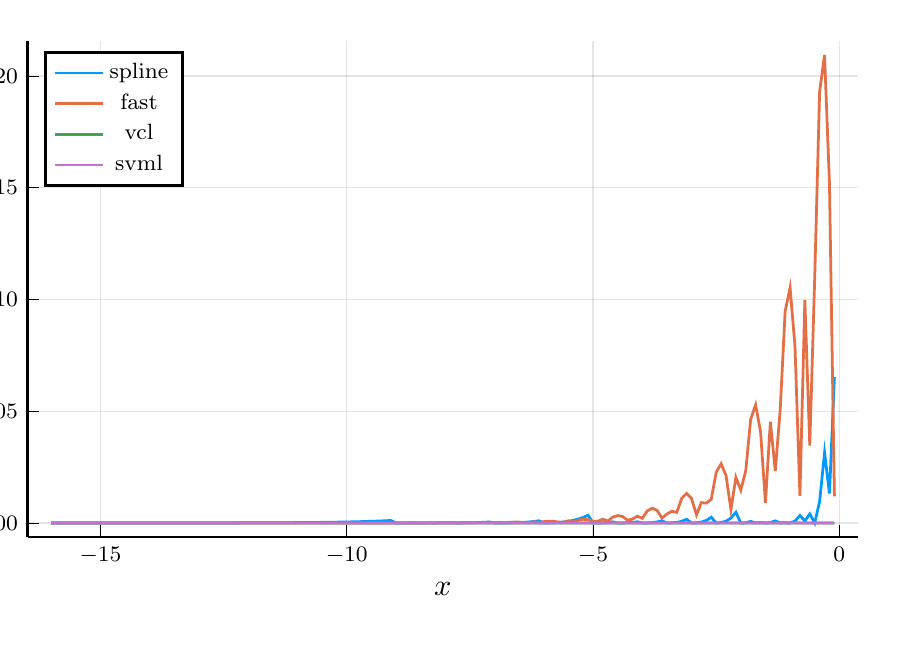
\begin{tikzpicture}[/tikz/background rectangle/.style={fill={rgb,1:red,1.0;green,1.0;blue,1.0}, fill opacity={1.0}, draw opacity={1.0}}, show background rectangle, trim axis left]
\begin{axis}[point meta max={nan}, point meta min={nan}, legend cell align={left}, legend columns={1}, title style={at={{(0.5,1)}}, anchor={south}, font={{\fontsize{14 pt}{18.2 pt}\selectfont}}, color={rgb,1:red,0.0;green,0.0;blue,0.0}, draw opacity={1.0}, rotate={0.0}, align={center}}, legend style={color={rgb,1:red,0.0;green,0.0;blue,0.0}, draw opacity={1.0}, line width={1}, solid, fill={rgb,1:red,1.0;green,1.0;blue,1.0}, fill opacity={1.0}, text opacity={1.0}, font={{\fontsize{8 pt}{10.4 pt}\selectfont}}, text={rgb,1:red,0.0;green,0.0;blue,0.0}, cells={anchor={center}}, at={(0.02, 0.98)}, anchor={north west}}, axis background/.style={fill={rgb,1:red,1.0;green,1.0;blue,1.0}, opacity={1.0}}, anchor={north west}, xshift={1.0mm}, yshift={-1.0mm}, width=\textwidth, height=0.65*\textwidth, scaled x ticks={false}, xlabel={$x$}, x tick style={color={rgb,1:red,0.0;green,0.0;blue,0.0}, opacity={1.0}}, x tick label style={color={rgb,1:red,0.0;green,0.0;blue,0.0}, opacity={1.0}, rotate={0}}, xlabel style={at={(ticklabel cs:0.5)}, anchor=near ticklabel, at={{(ticklabel cs:0.5)}}, anchor={near ticklabel}, font={{\fontsize{11 pt}{14.3 pt}\selectfont}}, color={rgb,1:red,0.0;green,0.0;blue,0.0}, draw opacity={1.0}, rotate={0.0}}, xmajorgrids={true}, xmin={-16.4770000357}, xmax={0.37700122570000083}, xticklabels={{$-15$,$-10$,$-5$,$0$}}, xtick={{-15.0,-10.0,-5.0,0.0}}, xtick align={inside}, xticklabel style={font={{\fontsize{8 pt}{10.4 pt}\selectfont}}, color={rgb,1:red,0.0;green,0.0;blue,0.0}, draw opacity={1.0}, rotate={0.0}}, x grid style={color={rgb,1:red,0.0;green,0.0;blue,0.0}, draw opacity={0.1}, line width={0.5}, solid}, axis x line*={left}, x axis line style={color={rgb,1:red,0.0;green,0.0;blue,0.0}, draw opacity={1.0}, line width={1}, solid}, scaled y ticks={false}, ylabel={err}, y tick style={color={rgb,1:red,0.0;green,0.0;blue,0.0}, opacity={1.0}}, y tick label style={color={rgb,1:red,0.0;green,0.0;blue,0.0}, opacity={1.0}, rotate={0}}, ylabel style={at={(ticklabel cs:0.5)}, anchor=near ticklabel, at={{(ticklabel cs:0.5)}}, anchor={near ticklabel}, font={{\fontsize{11 pt}{14.3 pt}\selectfont}}, color={rgb,1:red,0.0;green,0.0;blue,0.0}, draw opacity={1.0}, rotate={0.0}}, ymajorgrids={true}, ymin={-0.0006281340000000007}, ymax={0.02156593400000001}, yticklabels={{$0.000$,$0.005$,$0.010$,$0.015$,$0.020$}}, ytick={{0.0,0.005,0.01,0.015,0.02}}, ytick align={inside}, yticklabel style={font={{\fontsize{8 pt}{10.4 pt}\selectfont}}, color={rgb,1:red,0.0;green,0.0;blue,0.0}, draw opacity={1.0}, rotate={0.0}}, y grid style={color={rgb,1:red,0.0;green,0.0;blue,0.0}, draw opacity={0.1}, line width={0.5}, solid}, axis y line*={left}, y axis line style={color={rgb,1:red,0.0;green,0.0;blue,0.0}, draw opacity={1.0}, line width={1}, solid}, colorbar={false}]
    \addplot[color={rgb,1:red,0.0;green,0.6056;blue,0.9787}, name path={17}, draw opacity={1.0}, line width={1}, solid]
        table[row sep={\\}]
        {
            \\
            -16.0  1.12535176e-7  \\
            -15.9  1.2437064e-7  \\
            -15.8  1.3745074e-7  \\
            -15.7  1.5190662e-7  \\
            -15.6  1.6788269e-7  \\
            -15.5  1.8553914e-7  \\
            -15.4  2.0505253e-7  \\
            -15.3  2.2661797e-7  \\
            -15.2  2.5045168e-7  \\
            -15.1  2.7679175e-7  \\
            -15.0  3.0590232e-7  \\
            -14.9  3.3807447e-7  \\
            -14.8  3.7362986e-7  \\
            -14.7  4.1292503e-7  \\
            -14.6  4.5635247e-7  \\
            -14.5  5.0434767e-7  \\
            -14.4  5.573906e-7  \\
            -14.299999  6.160121e-7  \\
            -14.2  6.807983e-7  \\
            -14.099999  7.523987e-7  \\
            -14.0  8.315287e-7  \\
            -13.9  9.189817e-7  \\
            -13.799999  1.0156323e-6  \\
            -13.7  1.1224466e-6  \\
            -13.599999  1.2404957e-6  \\
            -13.5  1.3709591e-6  \\
            -13.4  1.5151447e-6  \\
            -13.299999  1.6744945e-6  \\
            -13.2  1.8506015e-6  \\
            -13.099999  2.045232e-6  \\
            -13.0  2.2603294e-6  \\
            -12.9  2.4980513e-6  \\
            -12.799999  2.7607746e-6  \\
            -12.699999  3.051129e-6  \\
            -12.599999  3.372017e-6  \\
            -12.499999  3.7266568e-6  \\
            -12.4  4.1185904e-6  \\
            -12.299999  4.551748e-6  \\
            -12.199999  5.0304616e-6  \\
            -12.099999  5.5595165e-6  \\
            -11.999999  6.1442183e-6  \\
            -11.9  6.7904075e-6  \\
            -11.799999  7.5045637e-6  \\
            -11.699999  8.293829e-6  \\
            -11.599999  9.166093e-6  \\
            -11.499999  1.0130103e-5  \\
            -11.4  1.1195489e-5  \\
            -11.299999  1.2372933e-5  \\
            -11.199999  1.3674212e-5  \\
            -11.099998  1.5112347e-5  \\
            -10.999999  1.6701717e-5  \\
            -10.899999  1.8458259e-5  \\
            -10.799999  2.0399519e-5  \\
            -10.699999  2.2544964e-5  \\
            -10.599998  2.4916048e-5  \\
            -10.499999  2.7536476e-5  \\
            -10.399999  3.0432524e-5  \\
            -10.299999  3.363312e-5  \\
            -10.199999  3.717036e-5  \\
            -10.099998  4.1079616e-5  \\
            -9.999999  4.5399975e-5  \\
            -9.899999  5.017475e-5  \\
            -9.799999  5.545164e-5  \\
            -9.699999  6.1283565e-5  \\
            -9.599998  6.772884e-5  \\
            -9.499998  7.4851974e-5  \\
            -9.399999  8.2724175e-5  \\
            -9.299998  9.142439e-5  \\
            -9.199999  0.00010103952  \\
            -9.099998  0.00011166598  \\
            -8.999998  0.0  \\
            -8.899999  3.3987000000001814e-7  \\
            -8.799998  6.624200000000173e-7  \\
            -8.699999  9.8551e-7  \\
            -8.599998  1.3421500000000122e-6  \\
            -8.499998  1.7820200000000057e-6  \\
            -8.399999  2.373220000000001e-6  \\
            -8.299998  3.2042600000000234e-6  \\
            -8.199999  4.386200000000009e-6  \\
            -8.099998  6.054880000000028e-6  \\
            -7.9999986  1.9999999974294053e-11  \\
            -7.8999987  3.9122999999997897e-7  \\
            -7.7999988  1.3012600000000384e-6  \\
            -7.6999984  2.9444600000000094e-6  \\
            -7.5999985  5.576140000000066e-6  \\
            -7.4999986  9.497069999999958e-6  \\
            -7.3999987  1.5058050000000102e-5  \\
            -7.2999988  2.2665360000000026e-5  \\
            -7.1999984  3.2786570000000034e-5  \\
            -7.0999985  4.595681000000001e-5  \\
            -6.9999986  0.0  \\
            -6.8999987  3.984999999999319e-7  \\
            -6.7999988  1.788599999999951e-6  \\
            -6.6999984  4.678500000000101e-6  \\
            -6.5999985  9.687600000000181e-6  \\
            -6.4999986  1.7559400000000027e-5  \\
            -6.3999987  2.9172899999999925e-5  \\
            -6.2999988  4.5558000000000013e-5  \\
            -6.199999  6.79112e-5  \\
            -6.0999985  9.761230000000006e-5  \\
            -5.9999986  0.0  \\
            -5.8999987  4.275700000000004e-6  \\
            -5.7999988  1.2355599999999689e-5  \\
            -5.699999  2.5753199999999955e-5  \\
            -5.5999985  4.628510000000011e-5  \\
            -5.4999986  7.610300000000011e-5  \\
            -5.3999987  0.00011772930000000011  \\
            -5.2999988  0.00017409589999999985  \\
            -5.199999  0.0002485858000000002  \\
            -5.0999985  0.00034508469999999965  \\
            -4.9999986  0.0  \\
            -4.8999987  4.820000000004335e-7  \\
            -4.7999988  5.361000000000601e-6  \\
            -4.699999  2.1187000000000636e-5  \\
            -4.599999  5.148049999999932e-5  \\
            -4.4999986  0.0  \\
            -4.3999987  2.43099999999892e-6  \\
            -4.2999988  9.37150000000081e-6  \\
            -4.199999  2.4687999999998406e-5  \\
            -4.099999  5.360299999999929e-5  \\
            -3.9999988  1.9999999989472883e-9  \\
            -3.8999987  3.0869999999988407e-6  \\
            -3.7999988  1.5489999999999948e-5  \\
            -3.6999989  4.45229999999977e-5  \\
            -3.5999987  9.974100000000041e-5  \\
            -3.4999988  0.0  \\
            -3.3999987  5.785000000001206e-6  \\
            -3.2999988  2.6707000000000813e-5  \\
            -3.1999989  7.463299999999756e-5  \\
            -3.099999  0.00016511999999999777  \\
            -2.9999988  0.0  \\
            -2.899999  7.680000000002962e-6  \\
            -2.7999988  3.931799999999652e-5  \\
            -2.6999989  0.00011432000000000109  \\
            -2.599999  0.000258170000000002  \\
            -2.4999988  0.0  \\
            -2.399999  1.939999999998887e-5  \\
            -2.2999988  8.252000000000259e-5  \\
            -2.1999989  0.00022217400000000553  \\
            -2.099999  0.00048124000000000777  \\
            -1.9999988  0.0  \\
            -1.8999988  6.86999999999216e-6  \\
            -1.7999989  6.9989999999992e-5  \\
            -1.6999989  1.940000000005826e-6  \\
            -1.5999988  2.0220000000015226e-5  \\
            -1.4999988  9.999999994736442e-9  \\
            -1.3999988  1.657000000002129e-5  \\
            -1.2999989  9.310000000001262e-5  \\
            -1.1999989  3.8499999999719314e-6  \\
            -1.0999988  8.710000000022866e-6  \\
            -0.9999988  2.9999999984209325e-8  \\
            -0.89999884  8.62400000000152e-5  \\
            -0.7999988  0.000335580000000002  \\
            -0.6999988  9.009999999998186e-5  \\
            -0.59999883  0.00040583000000005143  \\
            -0.4999988  0.0  \\
            -0.3999988  0.0009647699999999482  \\
            -0.29999882  0.0031470699999999185  \\
            -0.19999881  0.0013152600000000403  \\
            -0.09999881  0.006527399999999961  \\
        }
        ;
    \addlegendentry {spline}
    \addplot[color={rgb,1:red,0.8889;green,0.4356;blue,0.2781}, name path={18}, draw opacity={1.0}, line width={1}, solid]
        table[row sep={\\}]
        {
            \\
            -16.0  8.837860000000011e-10  \\
            -15.9  3.0786099999999855e-9  \\
            -15.8  1.0398400000000165e-9  \\
            -15.7  3.7815899999999954e-9  \\
            -15.6  5.004069999999999e-9  \\
            -15.5  4.546159999999991e-9  \\
            -15.4  2.230410000000019e-9  \\
            -15.3  2.136489999999991e-9  \\
            -15.2  5.510199999999985e-9  \\
            -15.1  2.5450000000000006e-9  \\
            -15.0  7.831519999999993e-9  \\
            -14.9  1.0056449999999959e-8  \\
            -14.8  8.898149999999993e-9  \\
            -14.7  3.998259999999971e-9  \\
            -14.6  5.0320999999999806e-9  \\
            -14.5  9.749900000000052e-9  \\
            -14.4  5.997699999999943e-9  \\
            -14.299999  1.617040000000004e-8  \\
            -14.2  2.017837000000003e-8  \\
            -14.099999  1.7372149999999914e-8  \\
            -14.0  7.032699999999925e-9  \\
            -13.9  1.1626130000000049e-8  \\
            -13.799999  1.7007099999999927e-8  \\
            -13.7  1.3759699999999903e-8  \\
            -13.599999  3.3298899999999994e-8  \\
            -13.5  4.042389999999995e-8  \\
            -13.4  3.3819399999999856e-8  \\
            -13.299999  1.2057900000000022e-8  \\
            -13.2  2.6460700000000038e-8  \\
            -13.099999  2.913699999999982e-8  \\
            -13.0  3.094240000000006e-8  \\
            -12.9  6.839720000000006e-8  \\
            -12.799999  8.085059999999989e-8  \\
            -12.699999  6.565839999999993e-8  \\
            -12.599999  1.994710000000019e-8  \\
            -12.499999  5.951599999999962e-8  \\
            -12.4  4.868159999999938e-8  \\
            -12.299999  6.851400000000024e-8  \\
            -12.199999  1.4015399999999995e-7  \\
            -12.099999  1.6142349999999996e-7  \\
            -11.999999  1.270750999999999e-7  \\
            -11.9  3.1239500000000364e-8  \\
            -11.799999  1.3259270000000042e-7  \\
            -11.699999  7.85740000000001e-8  \\
            -11.599999  1.4986850000000055e-7  \\
            -11.499999  2.8656500000000087e-7  \\
            -11.4  3.218280000000008e-7  \\
            -11.299999  2.450910000000008e-7  \\
            -11.199999  4.451899999999963e-8  \\
            -11.099998  2.9296799999999953e-7  \\
            -10.999999  1.2033299999999978e-7  \\
            -10.899999  3.2453800000000065e-7  \\
            -10.799999  5.845760000000022e-7  \\
            -10.699999  6.405439999999987e-7  \\
            -10.599998  4.70873999999998e-7  \\
            -10.499999  5.1859999999999195e-8  \\
            -10.399999  6.428909999999989e-7  \\
            -10.299999  1.6860400000000134e-7  \\
            -10.199999  6.96982999999997e-7  \\
            -10.099998  1.1903219999999945e-6  \\
            -9.999999  1.2727900000000051e-6  \\
            -9.899999  9.008429999999941e-7  \\
            -9.799999  2.6546999999999053e-8  \\
            -9.699999  1.4025499999999956e-6  \\
            -9.599998  1.9631000000000422e-7  \\
            -9.499998  1.4862059999999958e-6  \\
            -9.399999  2.419195000000012e-6  \\
            -9.299998  2.524640000000009e-6  \\
            -9.199999  1.715160000000004e-6  \\
            -9.099998  1.0610999999999618e-7  \\
            -8.999998  3.044500000000001e-6  \\
            -8.899999  1.170500000000161e-7  \\
            -8.799998  3.1490899999999994e-6  \\
            -8.699999  4.907739999999983e-6  \\
            -8.599998  4.998979999999996e-6  \\
            -8.499998  3.2475999999999924e-6  \\
            -8.399999  5.408799999999988e-7  \\
            -8.299998  6.579210000000021e-6  \\
            -8.199999  3.02329999999967e-7  \\
            -8.099998  6.639249999999992e-6  \\
            -7.9999986  9.938349999999983e-6  \\
            -7.8999987  9.880070000000025e-6  \\
            -7.7999988  6.10935999999999e-6  \\
            -7.6999984  1.7604600000000153e-6  \\
            -7.5999985  1.4162120000000026e-5  \\
            -7.4999986  1.6551999999999973e-6  \\
            -7.3999987  1.3932119999999983e-5  \\
            -7.2999988  2.009129999999996e-5  \\
            -7.1999984  1.9485399999999995e-5  \\
            -7.0999985  1.141149000000001e-5  \\
            -6.9999986  4.9203500000000655e-6  \\
            -6.8999987  2.954039999999991e-5  \\
            -6.7999988  5.360200000000112e-6  \\
            -6.6999984  2.911340000000002e-5  \\
            -6.5999985  4.054769999999996e-5  \\
            -6.4999986  3.835939999999988e-5  \\
            -6.3999987  2.1131800000000027e-5  \\
            -6.2999988  1.2725199999999957e-5  \\
            -6.199999  5.3628400000000145e-5  \\
            -6.0999985  1.4714500000000044e-5  \\
            -5.9999986  6.061070000000024e-5  \\
            -5.8999987  8.16838999999998e-5  \\
            -5.7999988  7.53549e-5  \\
            -5.699999  3.8725099999999905e-5  \\
            -5.5999985  3.139400000000013e-5  \\
            -5.4999986  9.654399999999962e-5  \\
            -5.3999987  3.720800000000038e-5  \\
            -5.2999988  0.0001257567000000001  \\
            -5.199999  0.00016431849999999984  \\
            -5.0999985  0.00014769499999999977  \\
            -4.9999986  7.00557000000001e-5  \\
            -4.8999987  7.504799999999943e-5  \\
            -4.7999988  0.0001720444999999994  \\
            -4.699999  8.954899999999953e-5  \\
            -4.599999  0.0002600555000000001  \\
            -4.4999986  0.00033001300000000053  \\
            -4.3999987  0.00028879300000000073  \\
            -4.2999988  0.00012463749999999836  \\
            -4.199999  0.00017525699999999984  \\
            -4.099999  0.0003027710000000003  \\
            -3.9999988  0.00020850999999999856  \\
            -3.8999987  0.0005363590000000001  \\
            -3.7999988  0.0006617460000000012  \\
            -3.6999989  0.000563240000000003  \\
            -3.5999987  0.00021716399999999886  \\
            -3.4999988  0.00040224999999999983  \\
            -3.3999987  0.0005244800000000008  \\
            -3.2999988  0.00047387900000000344  \\
            -3.1999989  0.0011033370000000028  \\
            -3.099999  0.0013248330000000044  \\
            -2.9999988  0.0010952139999999971  \\
            -2.899999  0.0003675549999999986  \\
            -2.7999988  0.0009108079999999991  \\
            -2.6999989  0.0008899399999999918  \\
            -2.599999  0.0010585150000000099  \\
            -2.4999988  0.0022640599999999983  \\
            -2.399999  0.0026480960000000026  \\
            -2.2999988  0.0021236899999999975  \\
            -2.1999989  0.000596366000000001  \\
            -2.099999  0.0020399200000000006  \\
            -1.9999988  0.0014691400000000077  \\
            -1.8999988  0.0023314899999999916  \\
            -1.7999989  0.004635200000000006  \\
            -1.6999989  0.005283559999999993  \\
            -1.5999988  0.00410452  \\
            -1.4999988  0.0009048400000000179  \\
            -1.3999988  0.0045280200000000215  \\
            -1.2999989  0.0023275600000000063  \\
            -1.1999989  0.005077949999999998  \\
            -1.0999988  0.009469000000000005  \\
            -0.9999988  0.010526650000000026  \\
            -0.89999884  0.00790436  \\
            -0.7999988  0.0012129499999999904  \\
            -0.6999988  0.009977400000000025  \\
            -0.59999883  0.0034593299999999827  \\
            -0.4999988  0.010957459999999974  \\
            -0.3999988  0.019300130000000082  \\
            -0.29999882  0.020937800000000006  \\
            -0.19999881  0.015161100000000038  \\
            -0.09999881  0.0011902500000000593  \\
        }
        ;
    \addlegendentry {fast}
    \addplot[color={rgb,1:red,0.2422;green,0.6433;blue,0.3044}, name path={19}, draw opacity={1.0}, line width={1}, solid]
        table[row sep={\\}]
        {
            \\
            -16.0  0.0  \\
            -15.9  0.0  \\
            -15.8  0.0  \\
            -15.7  0.0  \\
            -15.6  0.0  \\
            -15.5  0.0  \\
            -15.4  1.0000000009805158e-14  \\
            -15.3  0.0  \\
            -15.2  0.0  \\
            -15.1  0.0  \\
            -15.0  0.0  \\
            -14.9  0.0  \\
            -14.8  0.0  \\
            -14.7  0.0  \\
            -14.6  0.0  \\
            -14.5  0.0  \\
            -14.4  0.0  \\
            -14.299999  3.0000000002945693e-14  \\
            -14.2  0.0  \\
            -14.099999  0.0  \\
            -14.0  0.0  \\
            -13.9  0.0  \\
            -13.799999  0.0  \\
            -13.7  1.0000000015099114e-13  \\
            -13.599999  0.0  \\
            -13.5  0.0  \\
            -13.4  0.0  \\
            -13.299999  0.0  \\
            -13.2  0.0  \\
            -13.099999  0.0  \\
            -13.0  0.0  \\
            -12.9  0.0  \\
            -12.799999  1.999999998784658e-13  \\
            -12.699999  1.999999998784658e-13  \\
            -12.599999  0.0  \\
            -12.499999  0.0  \\
            -12.4  0.0  \\
            -12.299999  0.0  \\
            -12.199999  0.0  \\
            -12.099999  0.0  \\
            -11.999999  0.0  \\
            -11.9  0.0  \\
            -11.799999  0.0  \\
            -11.699999  0.0  \\
            -11.599999  0.0  \\
            -11.499999  0.0  \\
            -11.4  0.0  \\
            -11.299999  0.0  \\
            -11.199999  0.0  \\
            -11.099998  0.0  \\
            -10.999999  0.0  \\
            -10.899999  0.0  \\
            -10.799999  0.0  \\
            -10.699999  0.0  \\
            -10.599998  0.0  \\
            -10.499999  0.0  \\
            -10.399999  0.0  \\
            -10.299999  0.0  \\
            -10.199999  0.0  \\
            -10.099998  3.999999997569316e-12  \\
            -9.999999  0.0  \\
            -9.899999  0.0  \\
            -9.799999  0.0  \\
            -9.699999  0.0  \\
            -9.599998  0.0  \\
            -9.499998  0.0  \\
            -9.399999  0.0  \\
            -9.299998  0.0  \\
            -9.199999  0.0  \\
            -9.099998  0.0  \\
            -8.999998  0.0  \\
            -8.899999  0.0  \\
            -8.799998  0.0  \\
            -8.699999  0.0  \\
            -8.599998  0.0  \\
            -8.499998  9.999999987147026e-12  \\
            -8.399999  9.999999987147026e-12  \\
            -8.299998  0.0  \\
            -8.199999  0.0  \\
            -8.099998  0.0  \\
            -7.9999986  1.9999999974294053e-11  \\
            -7.8999987  0.0  \\
            -7.7999988  0.0  \\
            -7.6999984  0.0  \\
            -7.5999985  0.0  \\
            -7.4999986  0.0  \\
            -7.3999987  0.0  \\
            -7.2999988  0.0  \\
            -7.1999984  0.0  \\
            -7.0999985  0.0  \\
            -6.9999986  0.0  \\
            -6.8999987  0.0  \\
            -6.7999988  0.0  \\
            -6.6999984  0.0  \\
            -6.5999985  0.0  \\
            -6.4999986  2.0000000006820118e-10  \\
            -6.3999987  1.0000000003410059e-10  \\
            -6.2999988  0.0  \\
            -6.199999  0.0  \\
            -6.0999985  0.0  \\
            -5.9999986  0.0  \\
            -5.8999987  0.0  \\
            -5.7999988  2.999999996686209e-10  \\
            -5.699999  0.0  \\
            -5.5999985  0.0  \\
            -5.4999986  0.0  \\
            -5.3999987  0.0  \\
            -5.2999988  0.0  \\
            -5.199999  0.0  \\
            -5.0999985  0.0  \\
            -4.9999986  0.0  \\
            -4.8999987  0.0  \\
            -4.7999988  0.0  \\
            -4.699999  0.0  \\
            -4.599999  0.0  \\
            -4.4999986  9.999999994736442e-10  \\
            -4.3999987  0.0  \\
            -4.2999988  0.0  \\
            -4.199999  0.0  \\
            -4.099999  0.0  \\
            -3.9999988  1.9999999989472883e-9  \\
            -3.8999987  0.0  \\
            -3.7999988  0.0  \\
            -3.6999989  0.0  \\
            -3.5999987  1.9999999989472883e-9  \\
            -3.4999988  0.0  \\
            -3.3999987  0.0  \\
            -3.2999988  0.0  \\
            -3.1999989  2.9999999984209325e-9  \\
            -3.099999  0.0  \\
            -2.9999988  0.0  \\
            -2.899999  0.0  \\
            -2.7999988  0.0  \\
            -2.6999989  0.0  \\
            -2.599999  0.0  \\
            -2.4999988  0.0  \\
            -2.399999  0.0  \\
            -2.2999988  0.0  \\
            -2.1999989  0.0  \\
            -2.099999  0.0  \\
            -1.9999988  0.0  \\
            -1.8999988  0.0  \\
            -1.7999989  0.0  \\
            -1.6999989  0.0  \\
            -1.5999988  0.0  \\
            -1.4999988  0.0  \\
            -1.3999988  0.0  \\
            -1.2999989  0.0  \\
            -1.1999989  0.0  \\
            -1.0999988  0.0  \\
            -0.9999988  0.0  \\
            -0.89999884  0.0  \\
            -0.7999988  0.0  \\
            -0.6999988  0.0  \\
            -0.59999883  0.0  \\
            -0.4999988  0.0  \\
            -0.3999988  0.0  \\
            -0.29999882  0.0  \\
            -0.19999881  0.0  \\
            -0.09999881  0.0  \\
        }
        ;
    \addlegendentry {vcl}
    \addplot[color={rgb,1:red,0.7644;green,0.4441;blue,0.8243}, name path={20}, draw opacity={1.0}, line width={1}, solid]
        table[row sep={\\}]
        {
            \\
            -16.0  0.0  \\
            -15.9  0.0  \\
            -15.8  0.0  \\
            -15.7  9.999999983335378e-15  \\
            -15.6  2.0000000019610315e-14  \\
            -15.5  9.999999983335378e-15  \\
            -15.4  9.999999983335378e-15  \\
            -15.3  0.0  \\
            -15.2  0.0  \\
            -15.1  0.0  \\
            -15.0  3.0000000002945693e-14  \\
            -14.9  3.0000000002945693e-14  \\
            -14.8  3.999999998628107e-14  \\
            -14.7  3.0000000002945693e-14  \\
            -14.6  0.0  \\
            -14.5  0.0  \\
            -14.4  0.0  \\
            -14.299999  1.0000000004511202e-13  \\
            -14.2  9.99999999392329e-14  \\
            -14.099999  6.000000000589139e-14  \\
            -14.0  3.0000000002945693e-14  \\
            -13.9  0.0  \\
            -13.799999  0.0  \\
            -13.7  1.0000000015099114e-13  \\
            -13.599999  2.999999998176987e-13  \\
            -13.5  0.0  \\
            -13.4  0.0  \\
            -13.299999  0.0  \\
            -13.2  0.0  \\
            -13.099999  2.999999998176987e-13  \\
            -13.0  0.0  \\
            -12.9  3.0000000024121517e-13  \\
            -12.799999  1.999999998784658e-13  \\
            -12.699999  1.999999998784658e-13  \\
            -12.599999  9.99999999392329e-14  \\
            -12.499999  0.0  \\
            -12.4  3.999999997569316e-13  \\
            -12.299999  2.999999998176987e-13  \\
            -12.199999  3.999999997569316e-13  \\
            -12.099999  4.999999996961645e-13  \\
            -11.999999  0.0  \\
            -11.9  4.999999996961645e-13  \\
            -11.799999  0.0  \\
            -11.699999  0.0  \\
            -11.599999  0.0  \\
            -11.499999  2.000000000478724e-12  \\
            -11.4  1.5000000007825594e-12  \\
            -11.299999  0.0  \\
            -11.199999  9.99999999392329e-13  \\
            -11.099998  0.0  \\
            -10.999999  0.0  \\
            -10.899999  0.0  \\
            -10.799999  1.0000000027804608e-12  \\
            -10.699999  1.999999998784658e-12  \\
            -10.599998  0.0  \\
            -10.499999  9.99999999392329e-13  \\
            -10.399999  0.0  \\
            -10.299999  2.0000000055609216e-12  \\
            -10.199999  0.0  \\
            -10.099998  7.999999995138632e-12  \\
            -9.999999  5.000000000349777e-12  \\
            -9.899999  0.0  \\
            -9.799999  0.0  \\
            -9.699999  0.0  \\
            -9.599998  1.0000000000699553e-11  \\
            -9.499998  0.0  \\
            -9.399999  5.00000000712604e-12  \\
            -9.299998  1.0000000000699553e-11  \\
            -9.199999  1.0000000000699553e-11  \\
            -9.099998  0.0  \\
            -8.999998  0.0  \\
            -8.899999  0.0  \\
            -8.799998  0.0  \\
            -8.699999  2.0000000001399107e-11  \\
            -8.599998  2.0000000001399107e-11  \\
            -8.499998  9.999999987147026e-12  \\
            -8.399999  0.0  \\
            -8.299998  0.0  \\
            -8.199999  2.9999999988546133e-11  \\
            -8.099998  1.9999999974294053e-11  \\
            -7.9999986  0.0  \\
            -7.8999987  2.9999999988546133e-11  \\
            -7.7999988  0.0  \\
            -7.6999984  2.000000002850416e-11  \\
            -7.5999985  0.0  \\
            -7.4999986  1.0000000003410059e-10  \\
            -7.3999987  4.999999990863008e-11  \\
            -7.2999988  0.0  \\
            -7.1999984  5.999999997709227e-11  \\
            -7.0999985  0.0  \\
            -6.9999986  0.0  \\
            -6.8999987  0.0  \\
            -6.7999988  9.999999981726015e-11  \\
            -6.6999984  1.0000000003410059e-10  \\
            -6.5999985  0.0  \\
            -6.4999986  1.0000000003410059e-10  \\
            -6.3999987  0.0  \\
            -6.2999988  0.0  \\
            -6.199999  0.0  \\
            -6.0999985  0.0  \\
            -5.9999986  2.0000000006820118e-10  \\
            -5.8999987  3.0000000010230177e-10  \\
            -5.7999988  0.0  \\
            -5.699999  3.0000000010230177e-10  \\
            -5.5999985  0.0  \\
            -5.4999986  0.0  \\
            -5.3999987  2.999999996686209e-10  \\
            -5.2999988  4.999999997368221e-10  \\
            -5.199999  4.999999997368221e-10  \\
            -5.0999985  0.0  \\
            -4.9999986  6.999999998050233e-10  \\
            -4.8999987  0.0  \\
            -4.7999988  9.999999994736442e-10  \\
            -4.699999  9.999999994736442e-10  \\
            -4.599999  4.999999997368221e-10  \\
            -4.4999986  9.999999994736442e-10  \\
            -4.3999987  9.999999994736442e-10  \\
            -4.2999988  5.000000014715456e-10  \\
            -4.199999  0.0  \\
            -4.099999  9.999999994736442e-10  \\
            -3.9999988  0.0  \\
            -3.8999987  9.999999994736442e-10  \\
            -3.7999988  9.999999994736442e-10  \\
            -3.6999989  2.0000000024167353e-9  \\
            -3.5999987  1.9999999989472883e-9  \\
            -3.4999988  0.0  \\
            -3.3999987  0.0  \\
            -3.2999988  0.0  \\
            -3.1999989  7.000000003254403e-9  \\
            -3.099999  0.0  \\
            -2.9999988  3.999999997894577e-9  \\
            -2.899999  4.999999997368221e-9  \\
            -2.7999988  0.0  \\
            -2.6999989  3.999999997894577e-9  \\
            -2.599999  0.0  \\
            -2.4999988  1.500000000598245e-8  \\
            -2.399999  1.000000000861423e-8  \\
            -2.2999988  0.0  \\
            -2.1999989  3.999999997894577e-9  \\
            -2.099999  0.0  \\
            -1.9999988  0.0  \\
            -1.8999988  0.0  \\
            -1.7999989  2.000000001722846e-8  \\
            -1.6999989  9.999999994736442e-9  \\
            -1.5999988  0.0  \\
            -1.4999988  0.0  \\
            -1.3999988  0.0  \\
            -1.2999989  1.9999999989472883e-8  \\
            -1.1999989  0.0  \\
            -1.0999988  6.00000000239298e-8  \\
            -0.9999988  6.00000000239298e-8  \\
            -0.89999884  0.0  \\
            -0.7999988  2.9999999984209325e-8  \\
            -0.6999988  0.0  \\
            -0.59999883  0.0  \\
            -0.4999988  0.0  \\
            -0.3999988  3.0000000039720476e-8  \\
            -0.29999882  6.000000007944095e-8  \\
            -0.19999881  0.0  \\
            -0.09999881  5.999999996841865e-8  \\
        }
        ;
    \addlegendentry {svml}
\end{axis}
\end{tikzpicture}

        \caption{$\exp$ Errors}
    \end{figure}

    \backmatter
    \printglossaries
    \printbibliography[heading=bibintoc]
\end{document}
